\documentclass[a4paper,11pt,twoside,DIV10,english,numbers=noendperiod]{scrbook}
\usepackage[a4paper,left=3.5cm,right=2.5cm,bottom=3.5cm,top=3cm]{geometry}
%{report}

% ~~~~~~~~~~~~~~~my packages~~~~~~~~~~~`
% package for block diagrams
\usepackage{tikz}
\usepackage{pgf}
\usetikzlibrary{shapes,arrows}
\usetikzlibrary{arrows,automata}
\usetikzlibrary{positioning}
% Multiline comments
\usepackage{verbatim}
%\usepackage[llncsdoc]{llncsdoc}
\usepackage{makeidx}  % allows for indexgeneration
%\usepackage{fullpage}
\usepackage[english]{babel}
\usepackage{graphicx}
\usepackage{multirow}
\usepackage{rotating}
\usepackage[latin1]{inputenc}
\usepackage[numbers,square]{natbib}
\usepackage{scrhack}
%Kapitel�berschriften in Gro�buchstaben
\setkomafont{chapter}{\normalfont \scshape \Huge}
\setkomafont{section}{\normalfont \bfseries \LARGE}
\setkomafont{subsection}{\normalfont \bfseries \Large}
\setkomafont{subsubsection}{\normalfont \bfseries \large}
\setkomafont{paragraph}{\normalfont \bfseries \large}
%Pallanoid Schriftart verwenden
\usepackage{mathpazo}

%Auswahl der Schriftart erm�gliche, damit Titelpage in Times und Rest in Pazo
\usepackage[T1]{fontenc}
\newcommand{\changefont}[3]{
\fontfamily{#1} \fontseries{#2} \fontshape{#3} \selectfont}

\usepackage{scalefnt}
\usepackage{titlesec}
\usepackage{titletoc}
\titleformat{\chapter}[display]
{\mdseries\huge\scshape}
{	\filleft
	\begingroup
		\scalefont{3}
			{\bfseries{\thechapter}}
	\endgroup}
{0ex}
{%\titlerule
\vspace{1ex}%
\filright}
[\vspace{1ex}%
\titlerule]

% Leere Seite ohne Seitennummer, naechste Seite rechts
\newcommand{\blankpage}{
 \clearpage{\pagestyle{empty}\cleardoublepage}
}

% Keine einzelnen Zeilen beim Anfang eines Abschnitts (Schusterjungen)
\clubpenalty = 10000
% Keine einzelnen Zeilen am Ende eines Abschnitts (Hurenkinder)
\widowpenalty = 10000 \displaywidowpenalty = 10000

%\usepackage[pdftex]{graphicx,color}
\usepackage{amsmath,amssymb,subfigure}

% Zeilenabstand einstellen %
\renewcommand{\baselinestretch}{1.25}
%\usepackage{setspace}
%\onehalfspacing

% Floating-Umgebungen anpassen %
\renewcommand{\topfraction}{0.9}
\renewcommand{\bottomfraction}{0.8}

% Theorem-Umgebungen
\usepackage[amsmath,thmmarks]{ntheorem}

% Caption Packet
\usepackage[margin=0pt,font=small,labelfont=bf]{caption}

% URLs
\usepackage{url}

% Bibtex deutsch
%\usepackage{bibgerm}

%\usepackage{abstract}

% Algorithmen

\usepackage{float}
\usepackage[ pdftex, plainpages=false, pdfpagelabels, hypertexnames=true, linktocpage=true, bookmarksopen=true, bookmarksopenlevel=1] {hyperref}
\usepackage[chapter]{algorithm}
\usepackage{algorithmic}

\setcounter{equation}{0}
% Theorem-Optionen %
\theoremseparator{.}
\theoremstyle{change}
\newtheorem{theorem}{Theorem}[section]
\newtheorem{satz}[theorem]{Satz}
\newtheorem{lemma}[theorem]{Lemma}
\newtheorem{korollar}[theorem]{Korollar}
\newtheorem{proposition}[theorem]{Proposition}
% Ohne Numerierung
\theoremstyle{nonumberplain}
\renewtheorem{theorem*}{Theorem}
\renewtheorem{satz*}{Satz}
\renewtheorem{lemma*}{Lemma}
\renewtheorem{korollar*}{Korollar}
\renewtheorem{proposition*}{Proposition}
% Definitionen mit \upshape
\theorembodyfont{\upshape}
\theoremstyle{change}
\newtheorem{definition}[theorem]{Definition}
\theoremstyle{nonumberplain}
\renewtheorem{definition*}{Definition}
% Kursive Schrift
\theoremheaderfont{\itshape}
\newtheorem{notation}{Notation}
\newtheorem{konvention}{Konvention}
\newtheorem{bezeichnung}{Bezeichnung}
\theoremsymbol{\ensuremath{\Box}}
\newtheorem{beweis}{Beweis}
\theoremsymbol{}
\theoremstyle{change}
\theoremheaderfont{\bfseries}
\newtheorem{bemerkung}[theorem]{Bemerkung}
\newtheorem{beobachtung}[theorem]{Beobachtung}
\newtheorem{beispiel}[theorem]{Beispiel}
\newtheorem{problem}{Problem}
\theoremstyle{nonumberplain}
\renewtheorem{bemerkung*}{Bemerkung}
\renewtheorem{beispiel*}{Beispiel}
\renewtheorem{problem*}{Problem}

% Algorithmen anpassen %
\renewcommand{\algorithmicrequire}[1]{\textbf{Eingabe:}#1\\}
\renewcommand{\algorithmicensure}[1]{\textbf{Ausgabe:}#1\\}
\floatname{algorithm}{Algorithmus}
\renewcommand{\listalgorithmname}{Algorithmenverzeichnis}

%Silbentrennung
\hyphenation{De-zi-mal-trenn-zeichen In-stal-la-ti-ons-as-sis-tent Ist-Schwer-punkt-po-si-tion}

\newcommand{\modelica}[3]{\vspace*{.75cm}
													\begin{addmargin}[0.5cm]{0.5cm} 
														\begin{minipage}{\linewidth}
															\noindent\rule[1ex]{\textwidth}{1pt}\\
															\noindent{\textbf{#1}\hfill\footnotesize(\textit{Modelica}-Quelltext - Auszug aus \ref{#2} auf Seite \pageref{#2})\normalsize}\\
															\noindent\rule[1ex]{\textwidth}{1pt}														
															\begin{flushleft}
																\hangindent=0.5cm #3	\\
															\end{flushleft}															
															\noindent\rule[1ex]{\textwidth}{1pt}\\
														
														\end{minipage}
													\end{addmargin}
													%\vspace*{.75cm}
												 }

\begin{document}
%\raggedbottom
	%\frontmatter

	\setcounter{secnumdepth}{3}
	\setcounter{tocdepth}{3}

	%\pagestyle{headings}  % switches on printing of running heads
	\pagenumbering{roman}
	
	%Schriftart f�r Titelseite auf TIMES
	\changefont{ptm}{m}{n}
	
	
\begin{titlepage}

 \sffamily

 \vspace*{-2cm}

 \begin{minipage}{0.48\linewidth}
  
\includegraphics[width=1.0\textwidth]{Bilder/tud_logo_rgb}
 \end{minipage}
 
 \vspace*{5.7cm}
 %\begin{center}
 % \noindent{
 %\begin{minipage}{0.55\linewidth}
%	\hrulefill
 % \vspace{2.0cm}
% \end{minipage}}
 \hfil
 %\begin{minipage}{0.4\linewidth}
  % empty
 %\end{minipage}
 %\begin{minipage}{0.15\linewidth}
  % empty
 %\end{minipage}
 \hfil
 \begin{minipage}{0.7\linewidth}
  \begin{center}
    \Huge\textbf{Master Thesis}
  \end{center}
  \begin{center}
    \huge{Estimation of Underactuated Degrees of Freedom(DOF's) in Humanoid Robots}\\[3ex]
  \end{center}
  \vspace{0.75cm}
  \begin{center}
    \large{Rajesh Rajendran}\\
 
 \normalsize{rajesh.rajendran@tu-dortmund.de}\\[2ex]
    \large{\today}
  \end{center}
 \end{minipage}
 \hfil
 \begin{minipage}{0.05\linewidth}
  % empty
 \end{minipage}
 \begin{minipage}{0.55\linewidth}
% \vspace{2.0cm}
%  \hrulefill
 \end{minipage}
% \end{center}
 %\vspace*{2cm}

 \vfill
 			\rmfamily
 			\changefont{ppl}{m}{n}
 			\begin{table} [H]
				\centering
				\normalsize
				\begin{tabular}{p{0.53\textwidth}p{0.41\textwidth}}
					Examiner: & \\
					Name of first examiner & Name of second examiner\\
			  	&\\	
			  	Abteilung Informationstechnik\newline Institut f\"{u}r Roboterforschung  & Lehrstuhl des Zweitgutachters\newline Fakult\"{a}t f\"{u}r Informatik\\

			  \end{tabular}
			 \end{table}
			 
				\rmfamily
 				\changefont{ppl}{m}{n}

 \end{titlepage}
 
    %Schriftart wieder zur\"{u}ck auf pazo
    \changefont{ppl}{m}{n}



    \blankpage
    \newpage
    \tableofcontents
    \cleardoublepage

    \pagenumbering{arabic}
    \parindent 0pt
    % Buchstaben in Formeln bzw. Gleichungen sollten
% in einer Arbeit durchweg die gleiche Bedeutung haben.
% Um das zu unterst�tzen, die Schreibarbeit zu verringern,
% und Umbennungen zu vereinfachen sollten alle Bezeichner
% zentral in einer Datei als Makro definiert werden.

% Abk�rzungen
\newcommand{\IRF}{Institut f�r Roboterforschung}

% Formelvariablen
\newcommand{\Ri}[2]{R^{#1}_{#2}} % Rotationsmatrix von Frame #2 zu Frame #1
\newcommand{\Rv}[2]{R_v\left(#1, #2\right)} % Rotationsmatrix um beliebige Achse #1 bei Winkel #1

    %%%%%%%%%%%
    % Kapitel %
    %%%%%%%%%%%

    \chapter{Introduction}
\label{sec:einleitung}
The field of \emph{Robotics} have seen a tremendous development since the introduction of the term by \emph{Isaac Asimov} in 1940s. The fundamental components of robotic systems are mechanical structure, actuators, sensors and controller. Robotic systems range from simple \emph{Cartesian manipulator} to the complex \emph{Humanoids}. \emph{Industrial robots} are robots that are used in applications such as palletizing, material loading and unloading, part sorting, packaging etc. These robots usually operate in the structured environment whose geometrical or physical characteristics are known a priori. They are preprogrammed to execute the set of tasks. These robots have largely aided the automation of manufacturing processes in the industries. \emph{Mobile robots} that are used in the environments where human beings can hardly survive or be exposed to unsustainable risks are called \emph{Field robots}. These robots normally operate in the unstructured environments, where the geometry or physical characteristics are not known a priori. The mars rover \emph{Curiosity} is one such example. Locomotion in these robots is achieved either by wheels or by mechanical legs. The robots that navigate with mechanical legs are gaining importance, because they can navigate through the rugged terrain. The legged robots are biologically inspired structures equipped with six (hexapod-inspired from insects), four (quadrapod-inspired from animals) and two (biped-inspired from human) legs. The bipeds having the same kinematic structure as the humans are called \emph{Humanoids}. \emph{Toro (Torque controlled robot)} is the humanoid developed by Department of Robotics and Mechatronics at DLR. It is used as a platform to test advanced control concepts used for waling and balancing. \emph{Toro} was built as a biped walker shown in Figure \ref{fig:toro_biped}. Later in 2012 it have been equipped with the upperbody and hands and evolved into a humanoid. The present form of \emph{Toro} is shown in \ref{fig:toro_humanoid}.
\begin{figure}
	\centering
	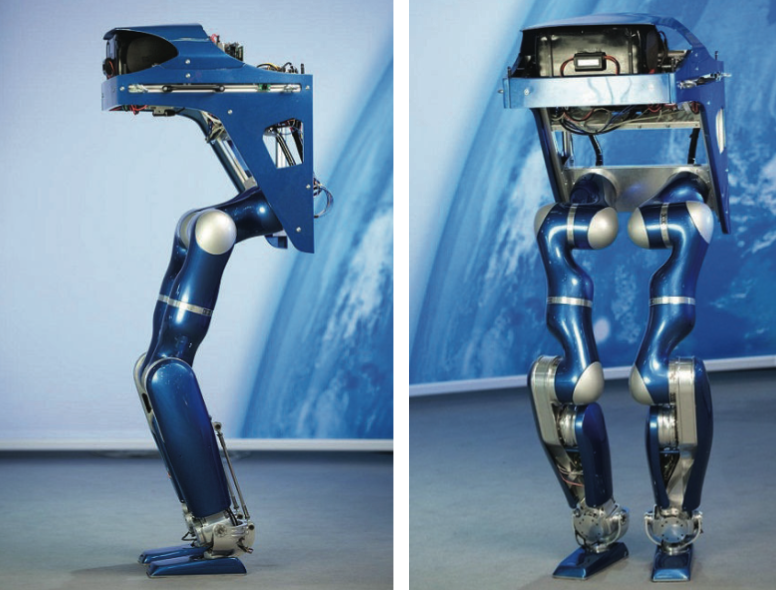
\includegraphics[scale=0.25]{Bilder/toro-biped}
	\caption{\emph{Toro} in biped form}
	\label{fig:toro_biped}
\end{figure}
\begin{figure}
\centering
	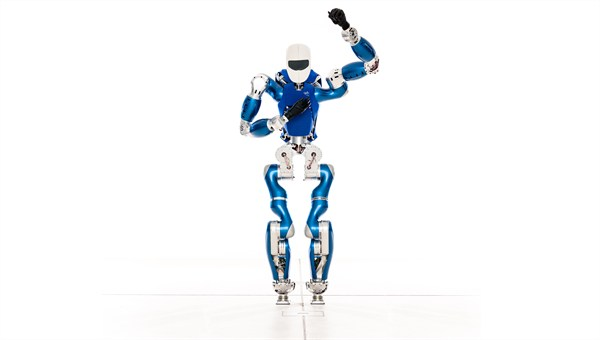
\includegraphics[trim=40mm 0mm 40mm 0mm,clip,scale=1]{Bilder/toropic}
	\caption{\emph{Toro} in humanoid form}
	\label{fig:toro_humanoid}
\end{figure}

\section{Motivation}
\begin{figure}
	\centering
	%\includegraphics[angle=-90,scale=0.65]{Bilder/walking_ctrl.pdf}
	%\pgfdeclarelayer{background}
%\pgfdeclarelayer{foreground}
%\pgfsetlayers{background,main,foreground}

% Define a few styles and constants
\tikzstyle{smallbox}=[draw, top color=white, bottom color=blue!20, text width=5em,text centered, minimum height=2.5em]
\tikzstyle{relationship} = [diamond,top color=white,bottom color=red!20,draw=red!50!black!100]
\tikzstyle{bigbox} = [smallbox,top color=white,fill=green!30,minimum height=25em,rounded corners]
\tikzstyle{input} = [coordinate]
\tikzstyle{sum} = [draw, fill=blue!20, circle, node distance=1cm]
\tikzstyle{output} = [coordinate]
\def\blockdist{3}
\def\edgedist{1.5}

\begin{tikzpicture}[node distance=2cm]
	\node (zmp)[smallbox] {ZMP};
	\node (com) [smallbox,below of=zmp,node distance=7cm] {COM};
	\node (zmp_sum) [sum,right of=zmp,node distance=3cm]{};
	\node (zmp_ctrl) [smallbox,below of=zmp_sum,node distance=2cm]{ZMP Controller};
	\node (ctrl_sum) [sum,below of=zmp_ctrl,node distance=1.5cm]{};
	\node (kin_res) [smallbox,right of=ctrl_sum,node distance=3cm]{Kinematic Resolution of COM Jacobian};
	\node (jnt_sum) [sum,right of=kin_res,node distance=2cm]{};
	\node (jnt_msr) [input,below of=jnt_sum,node distance=3.5cm]{};
	\node (zmp_calc) [smallbox,right of=zmp_sum,node distance=3cm]{ZMP Calculation};
	\node (com_div) [output,right of=com,node distance=1.5cm]{};
	\node (dxdt) [rectangle,fill=blue!20,above of=com_div,node distance=0.75cm]{$\frac{d}{dt}$};
	\node (com_sum) [sum,below of=zmp_sum,node distance=7cm]{};
	\node (com_ctrl) [smallbox,above of=com_sum,node distance=2cm]{COM Controller};
	\node (com_calc) [smallbox,below of=zmp_calc,node distance=7cm]{COM Calculation};
	\node (jnt_ctrl) [smallbox,right of=jnt_sum,node distance=1.5cm]{Joint Controller};
	\node (robot) [bigbox,right of=jnt_ctrl,node distance=2.5cm]{Real Biped Robot};
	
	\draw [->] (zmp) --node[above,pos=0.5]{\small{Des. ZMP}}(zmp_sum)node[below,pos=0.3]{$p^d$};
	\draw [->] (zmp) --node{}(com);
	\draw [-] (com) --node{}(com_div);
	\draw [->] (com_div) --node[below,pos=0.4]{\small{Des. COM}}node[above]{$c^d$}(com_sum);
	\draw [->] (com_calc) --node[below,pos=0.5]{\small{Act. COM}}node[above,pos=0.5]{$c$}node[above,pos=0.9]{$-$}(com_sum);
	\draw [->] (com_div) --node{}(dxdt);
	\draw [->] (com_sum) --node{}(com_ctrl);
	\draw [->] (dxdt) |-node[left,pos=0.3]{$\dot c^d$}(ctrl_sum);
	\draw [->] (com_ctrl) --node{}(ctrl_sum);
	\draw [->] (zmp_ctrl) --node[right,pos=0.9]{$-$}(ctrl_sum);
	\draw [->] (ctrl_sum) --node[above,pos=0.5]{\small{Control}}node[below,pos=0.5]{\small{input }$u_i$}(kin_res);
	\draw [->] (zmp_sum) --node{}(zmp_ctrl);
	\draw [->] (zmp_calc) --node[above]{\small{Act. ZMP}}node[below]{$p$}node[below,pos=0.9]{$-$}(zmp_sum);
	\draw [->] (kin_res) --node[below]{$q_d$}(jnt_sum);
	\draw [->] (jnt_sum) --node{}(jnt_ctrl);
	\draw [->] (jnt_msr) --node[left]{$q$}node[left,pos=0.9]{$-$}(jnt_sum);
	\draw [->] (jnt_ctrl)--node{}(robot);
	\draw [->] (robot.west)+(0,3.5) --node[above]{FTS}(zmp_calc.east);
	\draw [->] (robot.west)+(0,-3.5) --node[above,pos=0.3]{Joint Angles}node[below]{$q$}(com_calc);
	
	\end{tikzpicture}

	\vspace{0.5cm}
	\caption{A walking controlled scheme of humanoid robot}
	\label{fig:walk_ctrl}
\end{figure}
% Navigating the humanoids in the unknown environments and dynamic balancing of mechanical structure demands advanced control schemes. \\
The walking control of a humanoid requires the trajectory tracking while maintaining the dynamic balance of the whole structure. The Figure \ref{fig:walk_ctrl} shows a Zero moment point (ZMP) based humanoid walking control scheme \citep{choi07}. Zero moment point is a point on the surface of the foot about which the combination of inertial forces and gravity forces does not produce any net moment. It is useful for determining the dynamic stability of the robot. The ZMP of a foot is computed from the ground reaction forces measured by the FTS [Appendix \ref{sec:zmp}]. The COM in the Figure \ref{fig:walk_ctrl} represents the center of mass of the object. In this control scheme the trajectory tracking is done by controlling the COM, and the dynamic balance is maintained by controlling the ZMP of the robot. The ZMP and COM controllers are the high level controllers that drives the Kinematic resolution of COM block which computes the desired joint angles $q_d$. The joint angles are controlled by a low level joint controller.

\paragraph{Illustartion:}    
     \begin{figure}
	    \centering
    	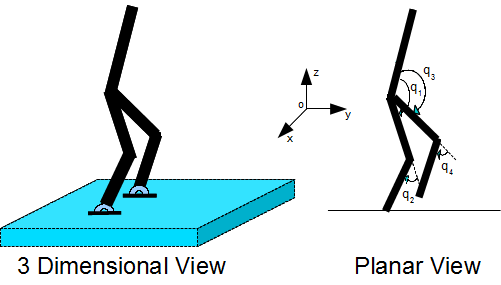
\includegraphics[scale=0.75]{Bilder/robot_flatfloor}
	    \caption{Humanoid robot standing on flat surface}	
	    \label{fig:flat_floor}
    \end{figure}
   Figure \ref{fig:flat_floor} shows a simplified two dimensional version of a humanoid robot standing on the flat surface. The COM of the robot is 
    \begin{equation}
    \label{eq:fwkin_flat}
    COM = f(q_1,q_2,q_3,q_4),
    \end{equation}
    where $f()$ is the forward kinematic function that determines the position of COM based on the joint anglse $q_i$. 
    \begin{figure}
	    \centering
    	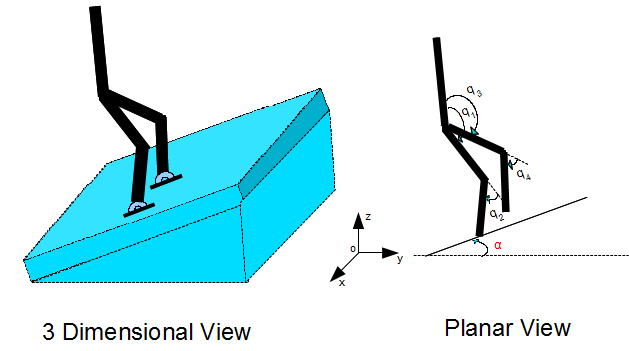
\includegraphics[scale=0.65]{Bilder/robot_slope}
	    \caption{Humanoid robot standing on a slope}	
	    \label{fig:slope}
    \end{figure}
The Figure \ref{fig:slope} shows a humanoid robot standing on the sloping surface. %In this case the COM computed by the forward kinematics function in Equation \ref{eq:fwkin_flat} will be wrong. 
%As we can see in the Figure \ref{fig:slope} there is an additional angle $\alpha$ acting between the surface of the real ground and the slope. There is no direct measurement available for this under-actuated degree of freedom. Failure to estimate this angle may lead to  tilting over an edge which might cause the robot to fall on the ground. Estimating this angle will help to achieve good balancing in the humanoid robot.
 The COM of the robot in Figure \ref{fig:slope} is given by $$COM = f(q_1,q_2,q_3,q_4,\alpha).$$  The angle $\alpha$ made by the robot with respect to the spatial frame (world coordinate frame) $O$ is not known. The computation of COM as a based on joint angles in Equation \ref{eq:fwkin_flat} will be incorrect in this case. Ignoring the angle $\alpha$ for COM computation will cause malfunctioning of the COM controller in Figure \ref{fig:walk_ctrl} and produces wrong control inputs $u_i$. The kinematic resolution of COM Jacobian block computes the desired joint angles $q_d$ assuming the robot is standing on a flat surface. When this joint trajectory executed by the controller it will cause the robot to tilt backwards. This will eventually lead to failure of the whole control scheme. This scenario motivates us to estimate the angle $\alpha$ in order to achieve robust control.  

\section{Problem Statement}
%    The focus of this thesis is estimation of under-actuated degrees of freedom of a humanoid robot.  Degrees of freedom of a robot is the number of joints present in the robot \citep{mur94}. In contrast to fixed base manipulators where the degrees of freedom is equal to number of joints in robot, the degrees of freedom of a humanoid robot is equal to sum of number of joints and degrees of freedom of a single rigid body. The under-actuated degrees of freedom of a humanoid robot are the degrees of freedom of a  rigid body.  A rigid body in three dimensional space can exhibit translational motion along \textbf{X,Y,Z} axes and rotational motion around these axes namely \emph{ roll, pitch ,yaw} as shown in Figure \ref{fig:rbody} in Chapter \ref{ch:multi_mdl}. 
	The angle $\alpha$ in Figure \ref{fig:slope} is the underactuated degree of freedom of the robot. 
% \paragraph{Underactuated degrees of freedom:}
    The term "underactuated degrees of freedom" means these degrees of freeodom are uncontrolled. They are the number of independent motions that can be exhibited by an object. For example in a two dimension (2D) space any object has 3 degrees of freedom, the object can translate along $X$ and $Y$ axes and rotate around $Z$ axis. The underactuated degrees of freedom are powered by the external forces acting on the object. For example the gravitational force makes the moon to rotate around the earth. It is not possible to directly control these degrees of freedom \citep{sab00}. In the industrial manipulators these degrees of freedom are constrained (by fixing the base to the ground), inorder to avoid complexity in control.
%%%%%%%%%%%%%%%%%%%%%%%%%%%%%%%%%%%%%%%%%%%%%%%%%%%%%%
 \begin{comment}
    \begin{figure}
    \begin{center}
    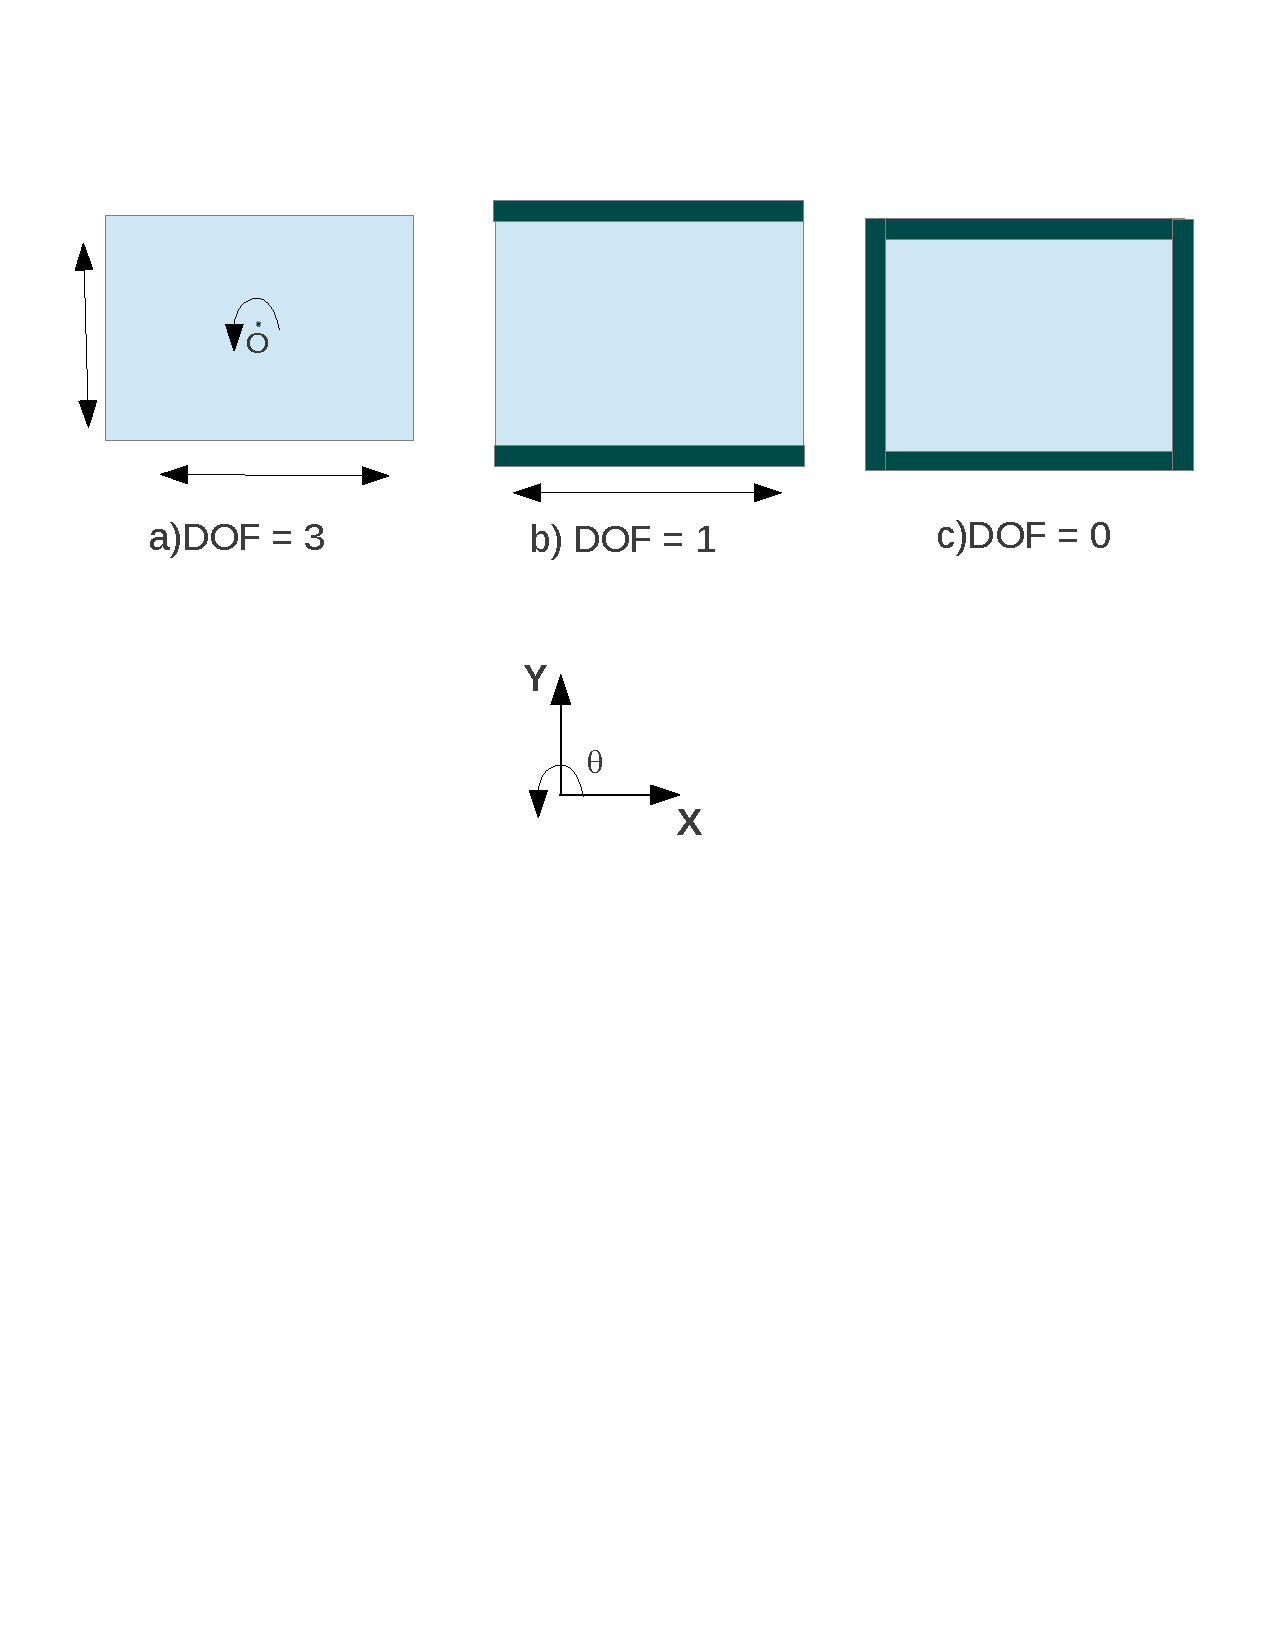
\includegraphics[trim = 10mm 130mm 10mm 20mm, scale = 0.75 ]{Bilder/dof2d.pdf}
    \caption{ Degrees of freedom of two dimensional object}
    \label{fig:dof_2d}
    \end{center}
    \end{figure}
    Figure \ref{fig:dof_2d} show how an object loses its degrees of freedom when it is constrained in 2 dimension space. In Figure \ref{fig:dof_2d} a) represents the unconstrained rectangular object free to move in space, b) represents the rectangular object constrained to move only along x axis and c) represents fully constrained rectangular object. 
    \end{comment}
%%%%%%%%%%%%%%%%%%%%%%%%%%%%%%%%%%%%%%%%%%%%%%%%%%%%%%%%%%%    
    %The ZMP of a foot is computed from the ground reaction forces measured by the FTS [Appendix \ref{sec:zmp}]. 
     
   The humanoid robots operates in a three dimensional (3D) space. The number of underactuated degrees of freedom of a 3D space is 6. 
   %When a humanoid is freely suspended (it is floating in air) it has six free degrees of freedom. But when it is constrained to its environment, the number of degrees of freedom decreases. 
   In this thesis we aim to estimate the motion of these degrees of freedom of a humanoid robot. The underactuated degrees of freedom are associated with a coordinate frame attached to the robot. In \emph{Toro} the coordinate frame is attached to the hip. As a result the state estimation problem involves estimating the motion of the hip coordinate frame. The motion parameters estimated are the position $p$, orientation $\theta$ and the body velocity $V^b$.

 \section{Methodology} 
The Kalman filter is an optimal state estimator for linear systems. The popular nonlinear extensions of Kalman filters used in practice are Extended Kalman filter(EKF) and Unscented Kalman filter(UKF). The usage of EKF for state estimation in humanoids is discussed in \citep{atk12}. \citep{bloe12} uses the EKF for state estimation in the hexapod robot. \citep{oli12} uses UKF for state estimation in humanoid robot. \citep{edg03} uses UKF for tracking the orientation of an inertial measurement unit. In this thesis the estimation problem is solved in both versions of Kalman filter. The results are compared based on accuracy of estimates and simulation time. Chapter \ref{ch:st_est} gives brief introduction to state estimation and describes the Kalman filtering algorithm. EKF and UKF algorithms are presented in Chapter \ref{ch:st_est}.

    Two different models are used for state estimation. They are the multibody system model and a simple model of  inertial measurement unit(IMU) \citep{bloe12}. The multibody system is a modelling formalism that is used to model the dynamic behaviour of a group of rigid bodies connected together to form the system. The state estimation problem using multibody system formulation is discussed in \citep{atk12}. In \citep{atk12}, the multibody system model of a simplified planar humanoid robot is used for predicting the states ahead of time. \citep{oli12} uses a multibody system model of the robot modelled using a maximal coordinate formulation scheme. The state estimation is performed separately on each link of the robot. Then the constraints due to the joints and contact are imposed on the estimates to get the true estimate of states. In this thesis, \emph{Toro} is modelled as a multibody system using minimum coordinate formulation or generalized coordinate formulation. State estimation of the multibody system involves estimation of position and velocity of the generalized coordinates. For instance, the model of \emph{Toro} have 31 generalized coordinates. The result of estimation problem will be 31 positions and 31 velocities of the generalized coordinates. Chapter \ref{ch:multi_mdl} deals with the modelling of multibody systems and its implementation in Kalman filtering algorithm. 
    
    A simplified motion model of IMU is discussed in \cite{bloe12}. In this paper, the EKF is used as sensor fusion algorithm for fusing IMU information with the kinematics of the hexapod. \citep{vis12} describes about an on-board odometry filter. The EKF is used to fuse the IMU motion model with the visual odometry and the kinematic odometry. The odometry filter is combined with vision based SLAM to obtain improved estimate of the motion model. An approach similar to \cite{bloe12} is implemented for humanoid robots. It is dealt in Chapter \ref{ch:simp_mdl}. The state estimation using this model involves predicting the position, orientation, translational velocity of the IMU sensor ahead of time. The position, orientation estimated are the under-actuated degrees of freedom and of the humanoid robot. This predicted states are updated by the kinematic information about the leg. State estimation using this model is more simpler than the multibody system. It is practically implemented on \emph{Toro}.

    %\chapter{Grundlagen}
\label{sec:Grundlagen}

	%% Diese Datei dient als Testseite für Befehle oder Formeln. 
% Alle hier eingegebenen können direkt am Anfang der Arbeit betrachtet werden.

%\begin{figure}
%\begin{center}
%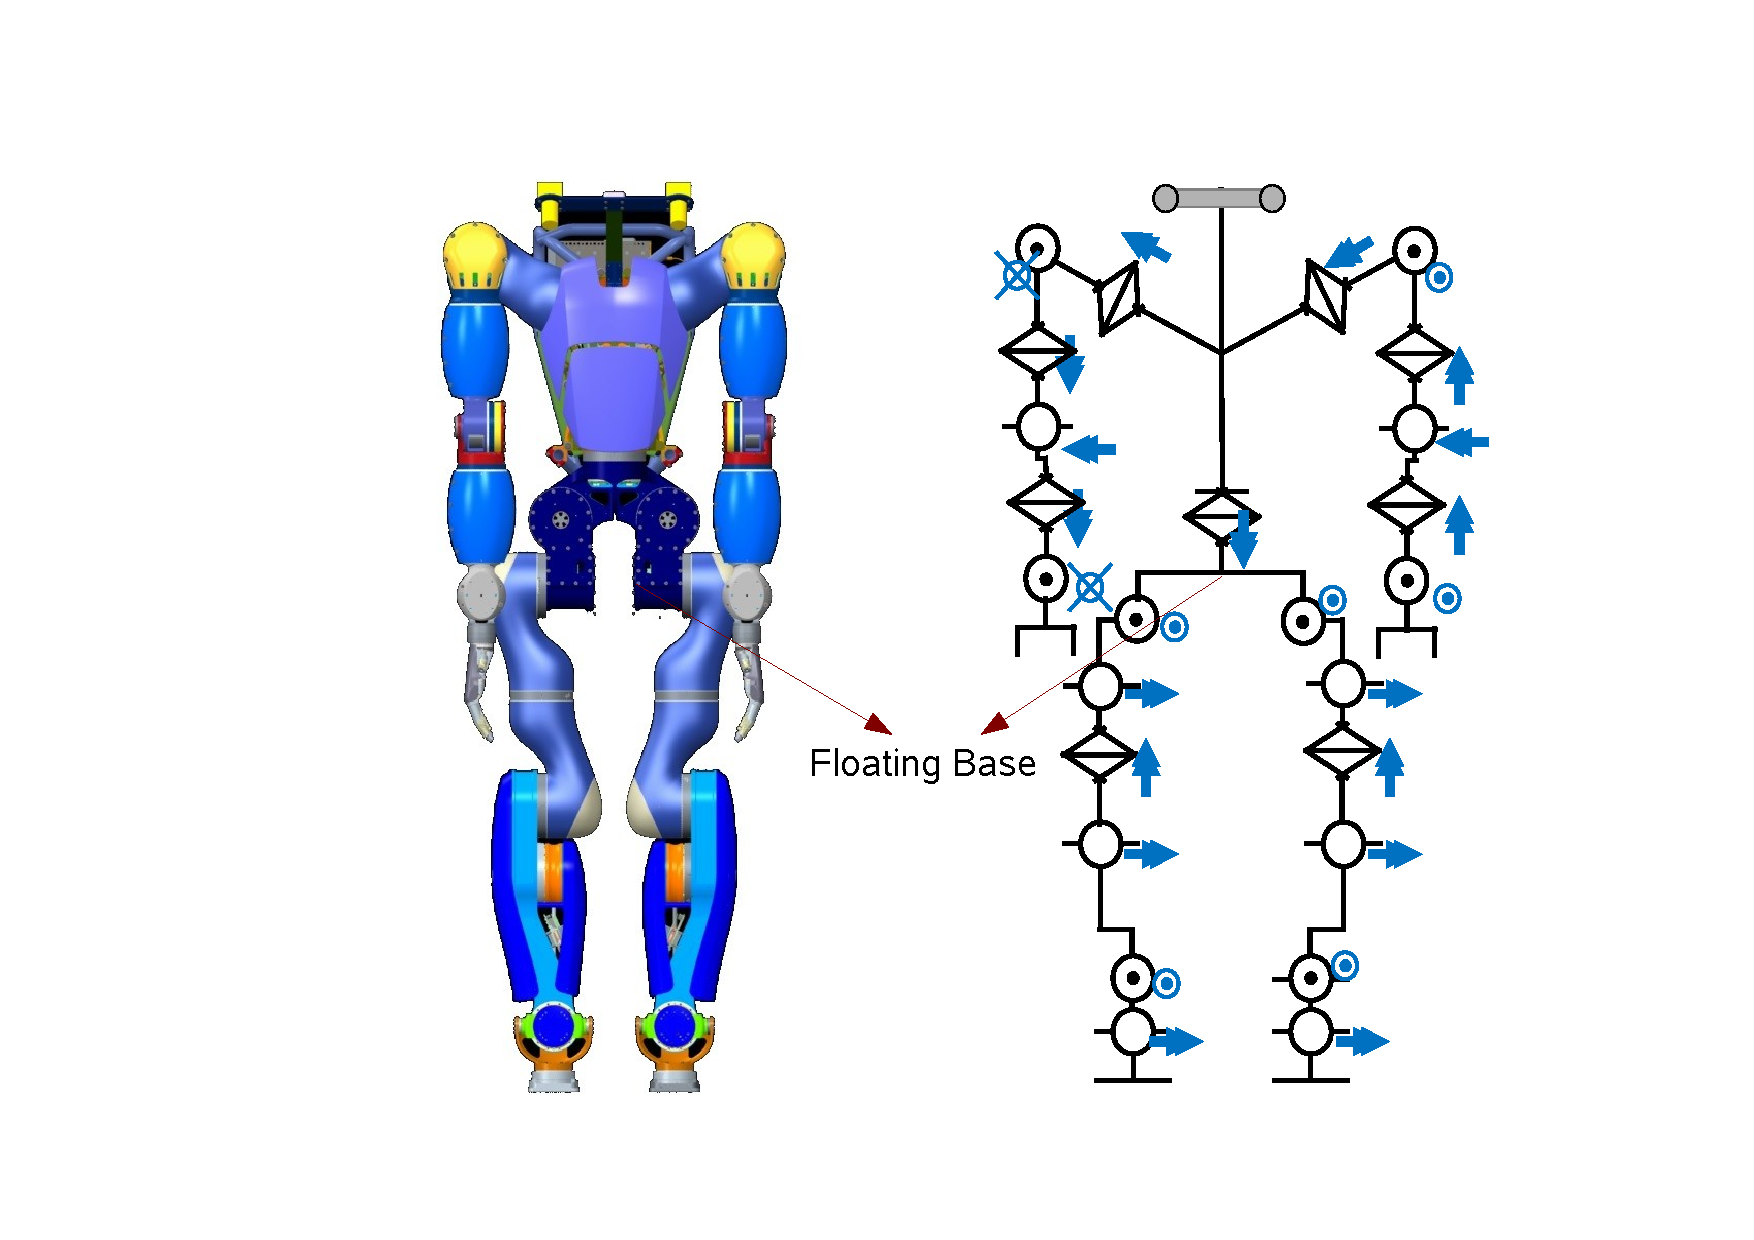
\includegraphics[scale=0.75]{Bilder/TORO_kinematic.pdf}
%\caption{test}
%\label{fig:foo}
%\end{center}
%\end{figure}
\begin{figure}
\tikzstyle{block} = [draw, fill=blue!20, rectangle, 
    minimum height=3em, minimum width=6em]
\tikzstyle{sum} = [draw, fill=blue!20, circle, node distance=1cm]
\tikzstyle{input} = [coordinate]
\tikzstyle{output} = [coordinate]
\tikzstyle{pinstyle} = [pin edge={to-,thin,black}]
\def\blockdist{2.3}
% The block diagram code is probably more verbose than necessary
\begin{tikzpicture}[auto, node distance=4cm,>=latex']
    % We start by placing the blocks
    \node [input, name=input] {};
    \node [sum, right of=input] (sum) {};
    \node [block, right of=sum] (controller) {Controller};
    \node [block, right of=controller, pin={[pinstyle]above:Disturbances},
            node distance=5cm] (system) {System};
    % We draw an edge between the controller and system block to 
    % calculate the coordinate u. We need it to place the measurement block. 
    \draw [->] (controller) -- node[name=u] {$u$} (system);
    \node [output, right of=system] (output) {};
    \node [block, below of= controller] (measurements) {Estimator};

    % Once the nodes are placed, connecting them is easy. 
    \draw [draw,->] (input) -- node {$r$} (sum);
    \draw [->] (sum) -- node {$e$} (controller);
    \draw [->] (system) -- node [name=y] {$y$}(output);
    \draw [->] (y) |- (measurements.base east);
    \draw [->] (u) |- (measurements.10);
    \draw [->] (measurements) -| node[pos=0.99] {$-$} 
        node [near end] {$\hat{x}$} (sum);
\end{tikzpicture}

\caption{Structure of state feedback controller}
\end{figure}
    \chapter{State Estimation}
\label{ch:st_est}
The state estimation is the principle of estimating the internal state(s) of the system from the measurement of input(s) and output(s) of the system. The knowledge of the internal state of the system will make the system easier to control. Figure \ref{fig:observer} shows the setup of state estimator in state feedback control loop.
\begin{figure}[h]
%  \centering
%  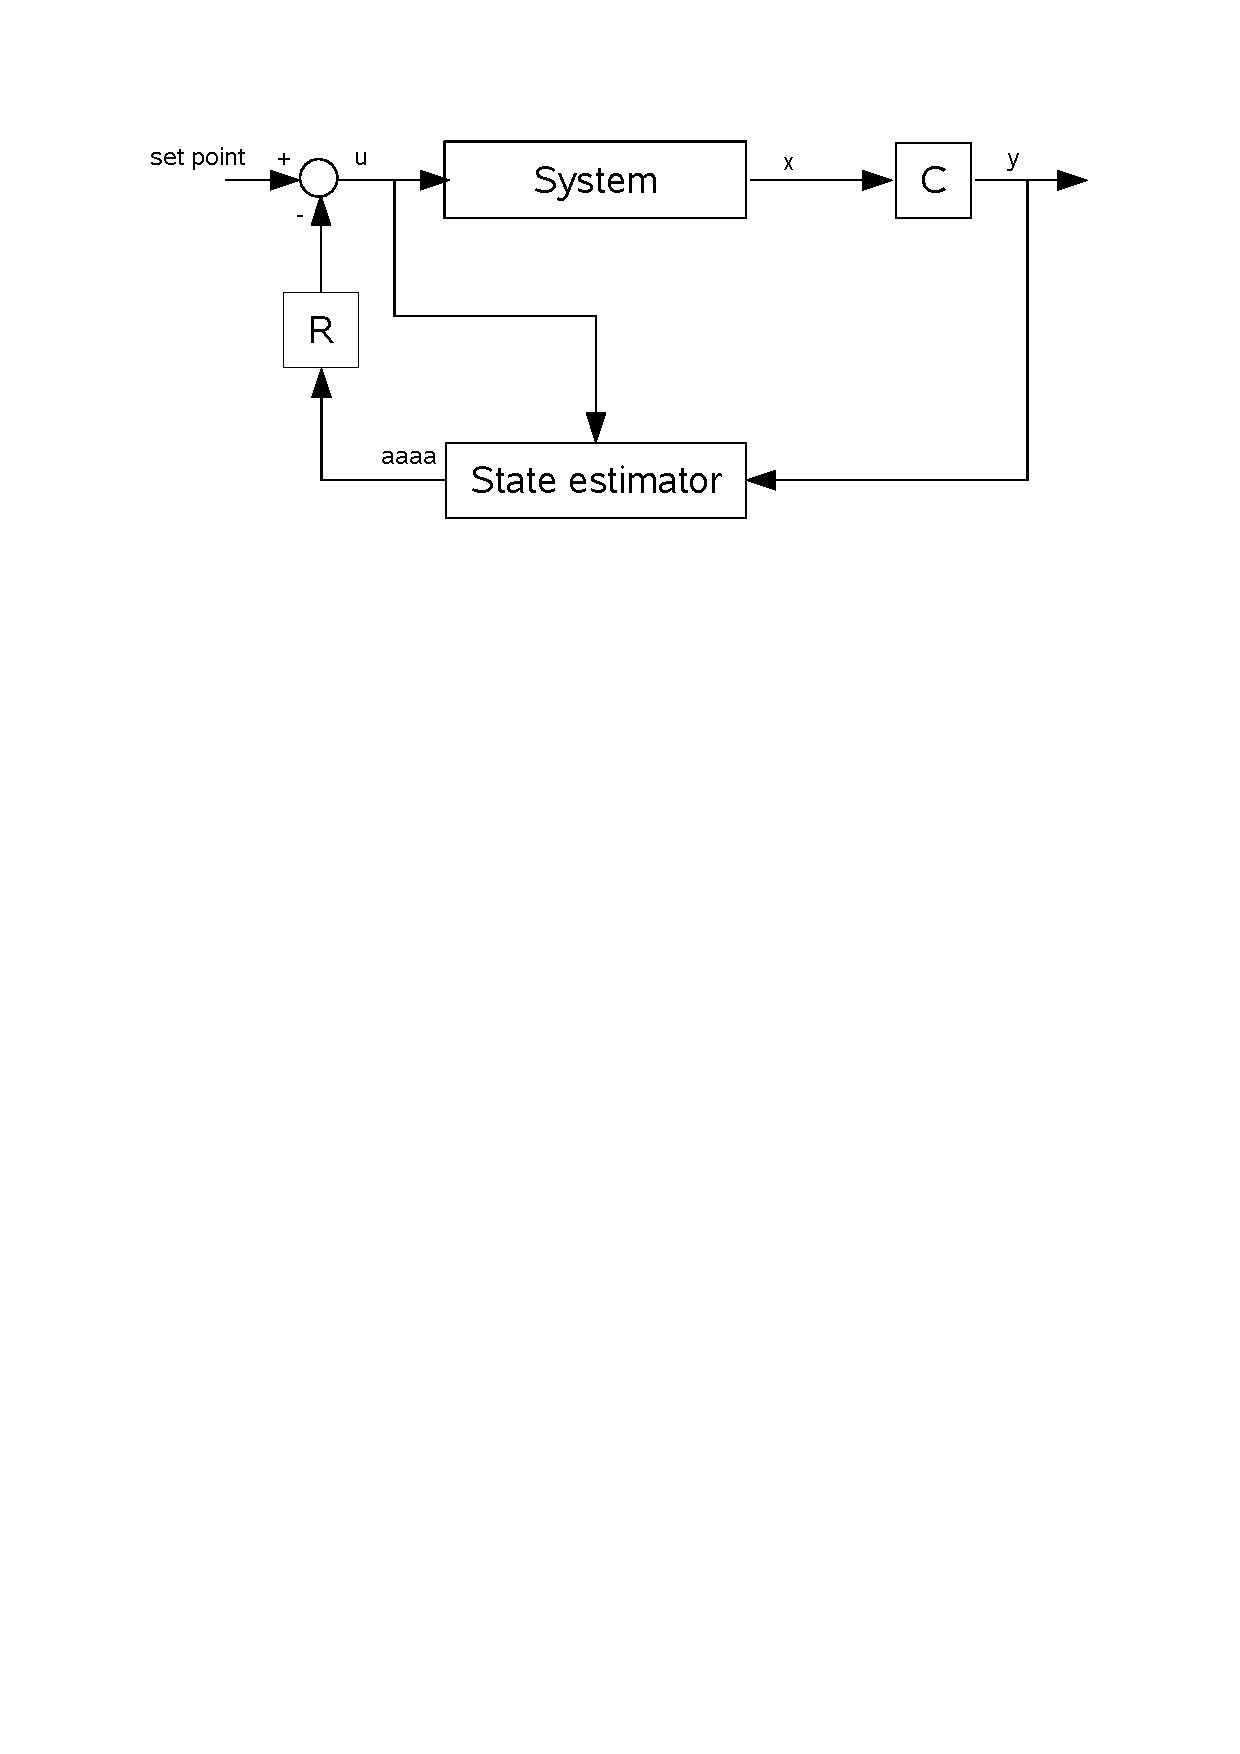
\includegraphics[trim = 10mm 200mm 20mm 20mm, clip,scale=0.80]{Bilder/system_observer.pdf}
\tikzstyle{block} = [draw, fill=blue!20, rectangle, 
    minimum height=3em, minimum width=6em]
\tikzstyle{sum} = [draw, fill=blue!20, circle, node distance=1cm]
\tikzstyle{input} = [coordinate]
\tikzstyle{output} = [coordinate]
\tikzstyle{pinstyle} = [pin edge={to-,thin,black}]
\def\blockdist{2.3}
% The block diagram code is probably more verbose than necessary
\begin{tikzpicture}[auto, node distance=4cm,>=latex']
    % We start by placing the blocks
    \node [input, name=input] {};
    \node [sum, right of=input] (sum) {};
    \node [block, right of=sum] (controller) {Controller};
    \node [block, right of=controller, pin={[pinstyle]above:Disturbances},
            node distance=5cm] (system) {System};
    % We draw an edge between the controller and system block to 
    % calculate the coordinate u. We need it to place the measurement block. 
    \draw [->] (controller) -- node[name=u] {$u$} (system);
    \node [output, right of=system] (output) {};
    \node [block, below of= controller] (measurements) {Estimator};

    % Once the nodes are placed, connecting them is easy. 
    \draw [draw,->] (input) -- node {$r$} (sum);
    \draw [->] (sum) -- node {$e$} (controller);
    \draw [->] (system) -- node [name=y] {$y$}(output);
    \draw [->] (y) |- (measurements.base east);
    \draw [->] (u) |- (measurements.10);
    \draw [->] (measurements) -| node[pos=0.99] {$-$} 
        node [near end] {$\hat{x}$} (sum);
\end{tikzpicture}
    \caption{State feedback controller with state estimator}
      \label{fig:observer}
\end{figure}

The state space equations of a nonlinear system is
\begin{equation}
\begin{split}
\label{eqn:nl_sys}
\dot{x}(t) &= f(x(t),u(t)) , x(t=0) = x_0 \\
y(t) &= g(x(t),u(t)),
\end{split}
\end{equation}

where $t$ is a scalar representing time, $x(t)$ represents the state vector, $u(t)$ represents the input vector and $y(t)$ represents the output vector of the system. The state $x(t)$,input $u(t)$ and output $y(t)$ depends on time $t$. The variable $x_0$ represents the vector of initial states $x(t=0)$ of the system. 
The state space equations of the state estimator is 
\begin{equation}
\begin{split}
\label{eqn:est_sys}
\dot{\hat{x}}(t) &= f(\hat{x}(t),u(t)) + K(y(t)-\hat{y}(t)) , \hat{x}(t=0) = \hat{x}_0  \\
\hat{y}(t) &= g(\hat{x}(t),u(t)),
\end{split}
\end{equation}
where $\hat{x}(t)$ \footnote{ The estimated states are represented by hat symbol at the top, inorder to differentiate them from the true states of the system. For example $\hat x_k$ represents the estimated states} is the state vector of estimator and $K$ is the estimator gain matrix.  A state estimator should satisfy the following properties \citep{gre01}:
\begin{itemize}
\item \textbf{Simulation property:} When the estimator and the system to be observed have same initial condition $x_0 = \hat{x}_0$, then it holds that $x(t) = \hat{x}(t) \forall t > 0 $
\item \textbf{Convergence property:} If $x_0 \neq \hat{x}_0$, then $x(t) - \hat{x}(t)$ tends to zero as $ t \rightarrow \infty $.
\end{itemize}

There are different methods for computing the estimator gain matrix $K$ in Equation \ref{eqn:est_sys}. The Luenberger observer has a deterministic way of computing the gain for linear systems. The sliding mode observer and the Kalman filter determines the gain matrix by minimizing the error between the estimates $\hat{x}$ and actual states $x$ \citep{kha02}.
    \section{Kalman Filter}
Kalman filter is a statistical state estimation algorithm which estimates the internal state of the system from the noisy measurements. It was designed by Rudolph E. Kalman in 1960 for discrete time linear systems. It is basically a predictor-corrector type estimator that is optimal in the sense that it minimizes the estimated error covariance. Since the measurements occur and the states are estimated at discrete points of time, it is easily implementable in digital computers. Kalman filters are extensively used in the area of autonomous and guided navigation.

\subsection{Kalman gain}
Given a discrete time linear system affected by random noise
\begin{equation}
\begin{split}
x_{k} &= Ax_{k-1} + Bu_k + w_{k-1}\\
y_k &= Hx_k + v_k
\end{split}
\end{equation}
where the random variables $w_k$,$v_k$ represent the process and measurement noise. Both the random variables are assumed to be zero mean Gaussian white noises. Let $Q,R$ be the covariance of process and measurement noise. Let us assume, 
\begin{equation}\label{eqn:kf_err}
e_k^- = x_k - \hat{x_k}^- 
\end{equation} be the error between the actual and predicted value of the state. The error covariance is given by 
\begin{equation}\label{eqn:kf_P}
P_k^- = E[e_k^- {e_k^-}^T]
\end{equation} Kalman filter corrects it estimate based on the predicted state and measured output data by 
\begin{equation} \label{eqn:kf_correct}
\hat{x_k} = \hat{x_k}^- + K(y_k - H\hat{x_k}^-)
\end{equation}
Kalman gain is computed by substituting Equation \ref{eqn:kf_correct} in Equation \ref{eqn:kf_err} to compute the $e_k^-$. Computed $e_k^-$ is substituted in Equation \ref{eqn:kf_P} and the expected values are computed to find the error covariance $P_k^-$. Finally \emph{K} is computed by taking the derivative of trace of $P_k^-$ and equating it to zero $$ \dfdx{trace(P_k^-)}{K} = 0 $$ solving the above equation for \emph{K}. One form of \emph{K} that minimizes Equation \ref{eqn:kf_correct}
\begin{equation} \label{eqn:kf_gain}
 K_k = P_k^- H^T(H P_k^- H^T + R)^{-1}
\end{equation}
From the Equation \ref{eqn:kf_gain} as measurement covariance \emph{R} approaches zero, Kalman gain \emph{K} lays more trust on actual measurement $y_k$. On the other hand if $P_k^-$ approaches zero, predicted measurement $H\hat{x_k}^-$ is trusted more.

\subsection{Extended Kalman filter}
Most of the real world estimation scenarios are non linear in nature. Kalman filter algorithm cannot be applied to the non linear systems. \emph{NASA Ames} devised a method to apply Kalman filter for non linear systems which is called the Extended Kalman filter(EKF). In EKF the non linear system is linearised by multivariate Taylor series expansion of the non linear function. 

Given a discrete time non linear system,
\begin{equation}
\begin{split}
x_{k} &= f(x_{k-1},u_k,w_{k-1})\\
y_k &= h(x_k,u_k,v_k)
\end{split}
\end{equation}
\emph{x,y} denotes the vector of system's state and output. \emph{w,v} represents the process and measurement covariance noise. \emph{f} is the non linear function that relates the previous state to the current state and \emph{h} is the non linear function that relates the output and state. 

In practice the individual values of noise $w_k$ and $v_k$ at each time step \emph{k} is not known. So one can compute the approximated state and measurement vector without them as 
\begin{equation}
\begin{split}
\hat{x}_k^- &= f(\hat{x}_{k-1},u_{k},0)\\
\hat{y}_k^- &= h(\hat{x}_k^-,u_{k},0)
\end{split}
\end{equation}
$\hat{x}_k^-$ and $\hat{y}_k^-$ are the \emph{priori} estimates of state and measurements at time step \emph{k} computed from \emph{posteriori} estimate of state $\hat{x}_{k-1}$ from previous time step \emph{k-1}.

$A_k$ and $H_k$ be the Jacobian matrices that results taking partial derivative of \emph{f} and \emph{h} with respect to \emph{x}  at time instant \emph{k}. $W_k$ and $V_k$ be the Jacobian matrices that results taking partial derivative of \emph{f} with respect to \emph{w} and \emph{h} with respect to \emph{v} at time step \emph{k}.
\begin{equation}
\begin{split}
A_k(i,j) &= \dfdx{f_i}{x_j}(\hat{x}_{k-1},u_k,0)\\
C_k(i,j) &= \dfdx{h_i}{x_j}(\hat{x}_k^-,u_k,0)\\
W_k(i,j) &= \dfdx{f_i}{w_j}(\hat{x}_{k-1},u_k,0)\\
V_k(i,j) &= \dfdx{h_i}{v_j}(\hat{x}_k^-,u_k,0)\\
\end{split}
\end{equation}
At each time step these Jacobian matrices are evaluated with current predicted states $\hat{x}_k^-$.
\subsubsection{Algorithm}
\textbf{Predict}
\begin{equation}
\begin{split}
%\text{Project the state}\\
\hat{x}_k^- &= f(\hat{x}_{k-1},u_k,0)\\
%\text{Procject the covarience}\\
P_k^- &= A_kP_{k-1}A_k^T + W_kQ_{k-1}W_k^T\\
\end{split}
\end{equation}
\textbf{Correct}\\
\begin{equation}
\begin{split}
K_k &= P_k^-H^T(H_kP_k^-H_k^T + V_kR_kV_k^T)^{-1}\\
\hat{x}_k &= \hat{x}_k^- + K_k(y_k-h(x_k^-,u_k,0))\\
P_k &= (I- K_kH_k)P_k^-
\end{split}
\end{equation}
% The result of th It has to be extended is  non-linear systems by extending the actual algorithm. This type of kalman filter algorithms %are called Extended kalman filters. There are also a new class of kalman filter algorithm which works on Bayasian principle, they are %called unscented Kalman filters.
\subsection{Unscented Kalman filter}
    %\input{Kapitel/Grundlagen/dpendulum.tex}
    %\def\dfdx#1#2{\frac{\partial {#1}}{\partial {#2}}}
\chapter{Multi body system model}
\label{chap:multi_mdl}
A multibody system model describes the dynamics of the group of interconnected rigid bodies that exhibits translational and rotational displacement. In this chapter the multi body system model of \emph{Toro} is derived and it is used as the prediction model in EKF.

\section{Multi body system}
The humanoid robots consists of group of rigid bodies(links) connected together by set of joints. Joints are mechanical components that connects two or more rigid bodies(links) and constraint their motion. Human beings are able to produce a motion with the help of the muscular system, where as the humanoids are driven by electric, hydraulic or pneumatic actuators, that apply torques to the joints of the robot which in turn produces the motion \cite[Chapter 2]{mur94}. The motion of bodies is described by their kinematic behaviour but the dynamic behaviour results from the equilibrium of applied froces and the rate of change of momentum. The dynamics of a robot describes how the robot moves in response to the actuator forces or torques. The dynamics of a multi body system(robot) is described by the equations of motion. In general there are several approaches in deriving equations of motion of rigid body dynamic system. One such approach is by deriving Lagrange equation. Lagrangian analysis relies on the energy properties of the mechanical system to derive the equations of motion. Lagrangian \emph{L} is defined as the difference between kinetic and potential energy of the system. Lagrangian \emph{L} is $$ L(q,\dot{q}) = T(q,\dot{q}) - V(q),$$ 
where \emph{q} represents the vector of joint angles, $\dot{q}$ is the vector of angular velocities of the joints, the kinetic and potential energies are represented by \emph{T} and \emph{V}. The joint angles \emph{q} is called the generalized coordinates of the system as the joint angles uniquely determines the position of rigid bodies in the system.

The equations of motion for a rigid body system in generalized coordinates $q \in \Re^m $ is given by
\begin{align}
\frac{d}{dt} &\dfdx{L}{\dot{q}} - \dfdx{L}{q_i} = \Gamma_i && i=1,....,m,
\end{align}
where $\Gamma_i$ is the external force acting on the $i^{th}$ generalized coordinate \cite[Chapter 4]{mur94}.
Simplifying and rearranging the above equation will result in the general formulation of equations of motion of a multi body system. It is given by
\begin{equation}
\label{eq:dyn_mul_bdy}
M(q)\ddot{q}+C(q,\dot{q})\dot{q}+g(q) = \tau + \tau_{ext},
\end{equation}
where \emph{M(q)} is the generalized inertia matrix, $C(q,\dot{q})$ is the matrix representing Coriolis and centrifugal forces, \emph{g(q)} is the gravity vector acting on the system and $\tau$ is the actuator torque applied to the joints $\tau_{ext}$ is the external torque acting on the system.

Rearranging the Equation \ref{eq:dyn_mul_bdy} results in the forward dynamics equation of the multibody system. Forward dynamics equation is the relation between the acceleration of the multi body system in repsonse to the forces and torques acting on the system.
\begin{equation}
    \label{eq:fwdyn}
    \ddot{q} = M(q)^{-1} (- C(q,\dot{q})\dot{q} -g(q) + \tau + \tau_{ext})
\end{equation}
\begin{itemize}
\item Inverted Double Pendulum model
\end{itemize}
\section{Inverted Double Pendulum model} 
\begin{figure}[H]
	\centering
	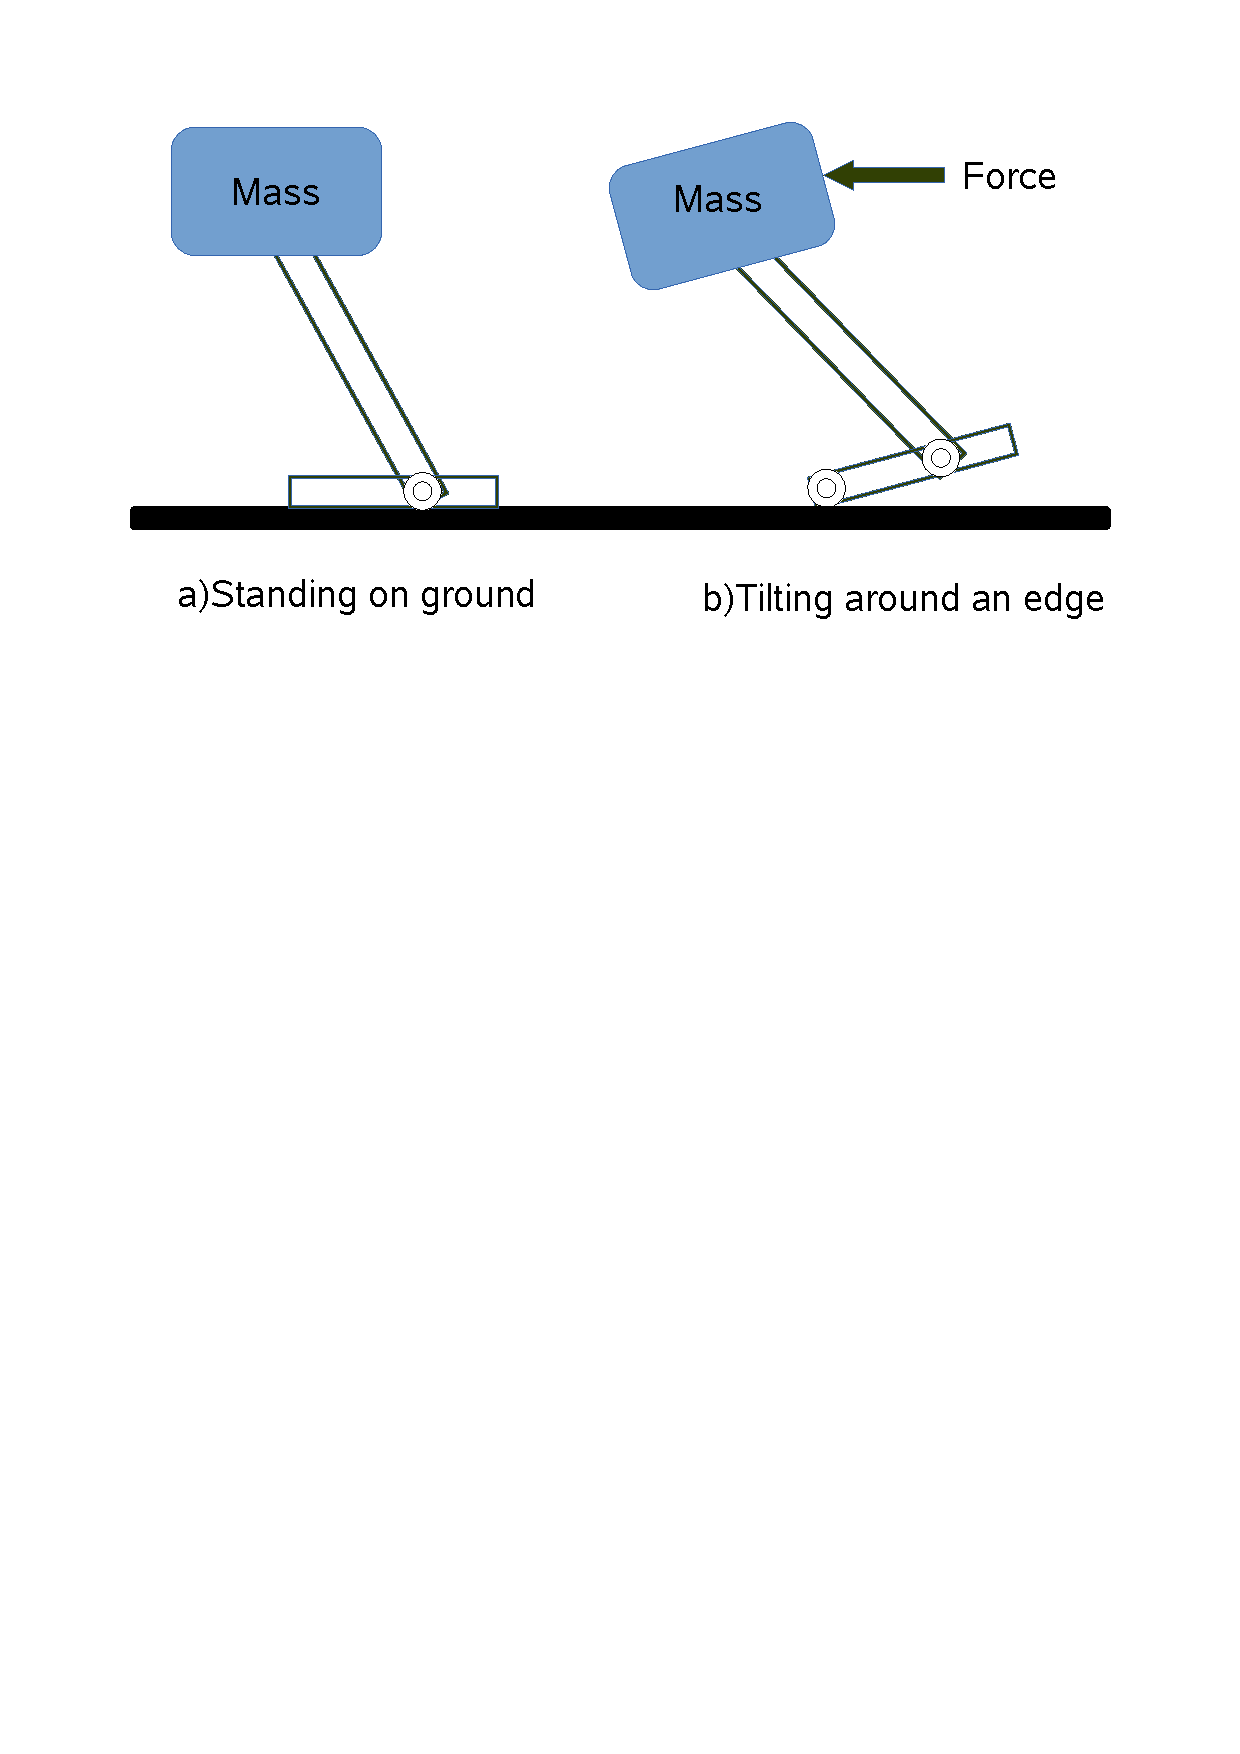
\includegraphics[trim = 0mm 180mm 0mm 10mm, scale=0.50]{Bilder/simp_uactcase.pdf}
	\caption{A simplified humanoid robot standing on one foot}
	\label{fig:idp_scene}
\end{figure}
Inorder to check the feasibility of solving the state estimation problem with the available measurements, a preliminary subproblem is formulated. Since we are interested in estimating the underactuated degrees of freedom, we have to consider the senario where these underactuated degrees of freedom are action on the robot. Let us consider the senario where the robot is tilting around an edge of the foot by applying some external force as shown in Figure \ref{fig:idp_scene}.b. Figure \ref{fig:idp_scene} shows a simplified version of a humanoid robot standing on one leg. All the joints other that ankle joint of the robot are assumed to remain static(joints does not produce any motion) throughout the experiment. The kinematics of the robot is simplified to one joint on the ankle connecting the whole body with the foot as shown in \ref{fig:idp_scene}.a. The kinematics of \emph{Toro} is shown in Figure \ref{fig:toro_kin}. The mass block in the Figure \ref{fig:idp_scene} represents the inertia of upperbody. The inertia of leg is incorporated in the link connceting upperbody and foot. 

When robot is tilting around an edge of the foot as shown in Figure \ref{fig:idp_scene}.b, we assume there is an imaginary joint located at the edge of the foot around which the robot tilts. Figure \ref{fig:idp_scene}.b resmbles an inverted double pendulum in Figure \ref{fig:idp}.
\begin{figure}[H]
	\centering
	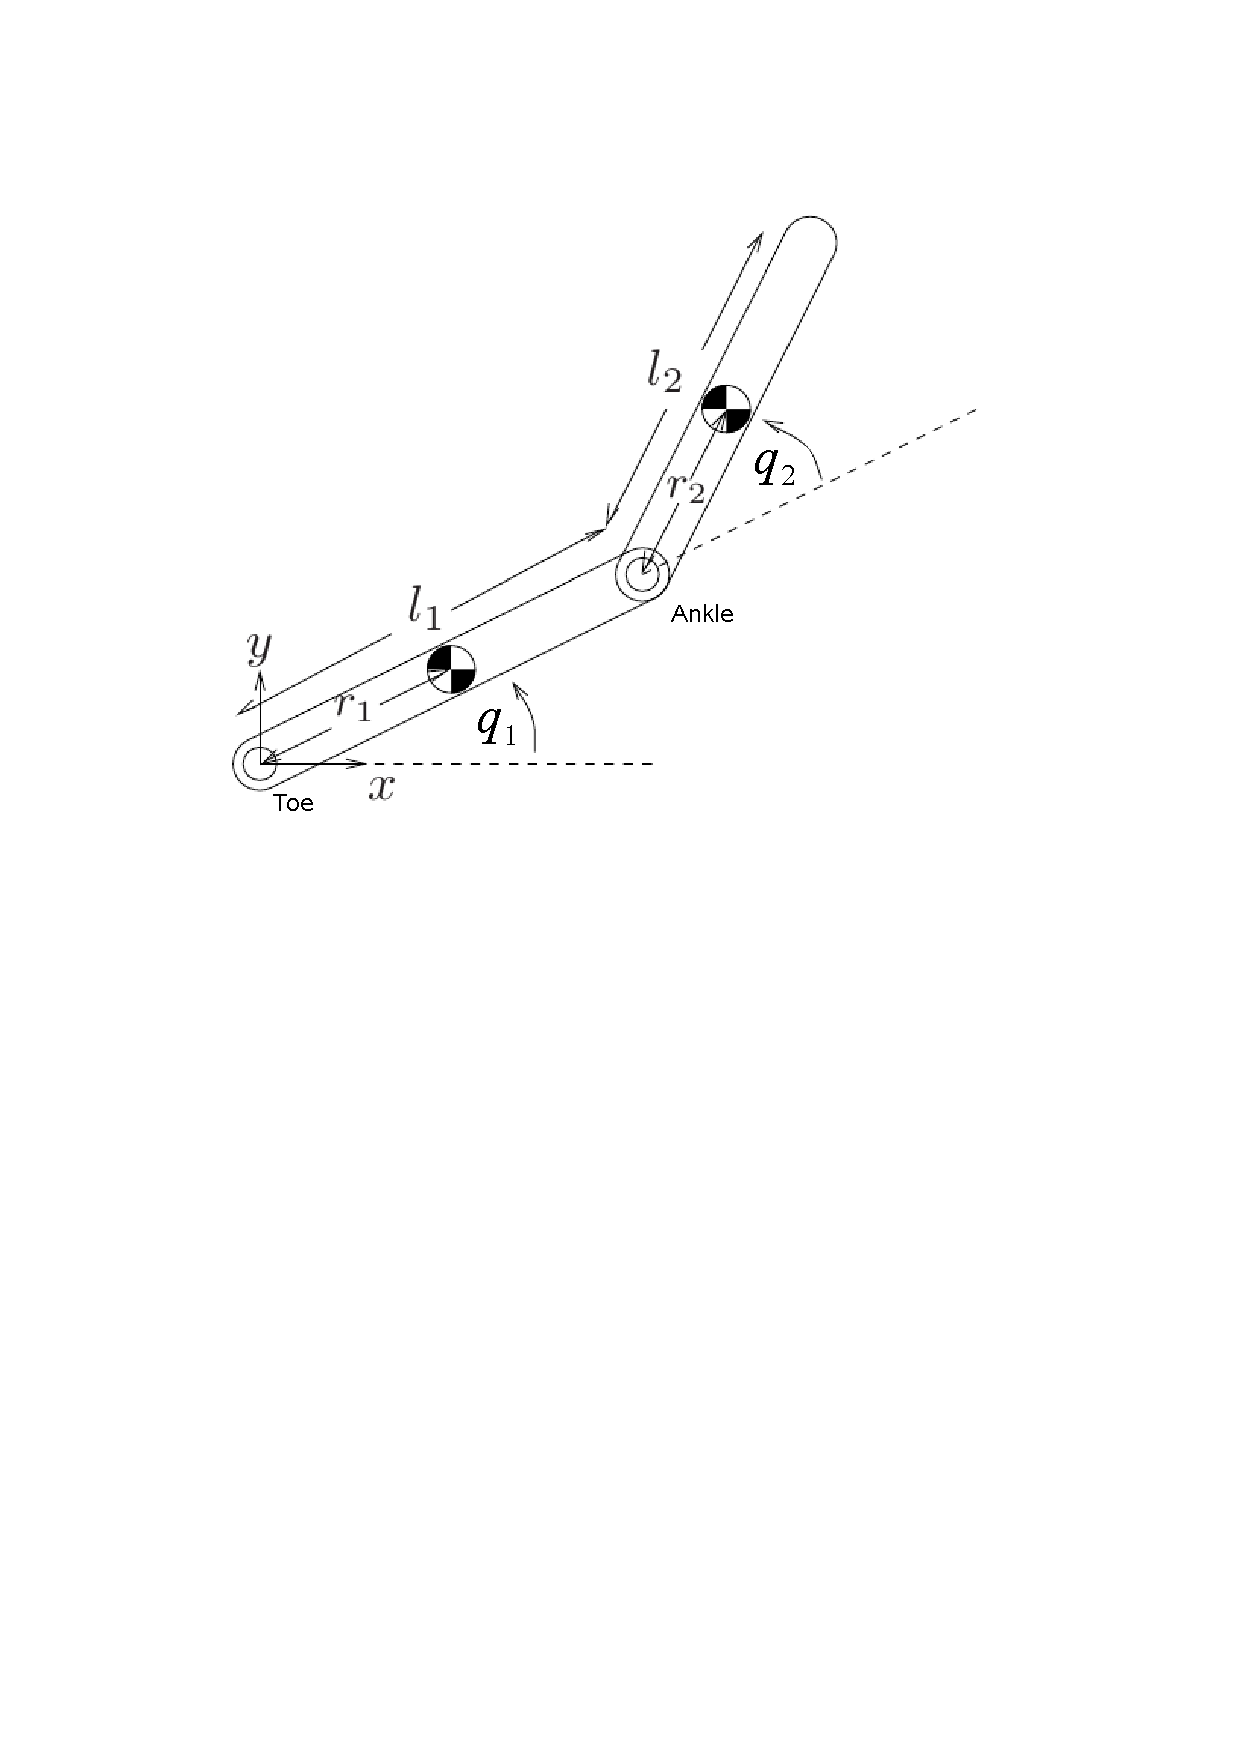
\includegraphics[trim= 0mm 150mm 0mm 0mm, scale=0.65]{Bilder/inv_db_pend.pdf}
	\caption[Inverted Double Pendulum]{Inverted Double Pendulum \footnotemark}
	\label{fig:idp}
\end{figure}
\footnotetext{Image source: A mathematical introduction to robotic manipulation \cite[Chapter 4, Page 164]{mur94}}
 The inverted double pendulum shown in Figure \ref{fig:idp} consists two links of length $l_1$ and $l_2$. The distance between center of mass of link 1 from the toe joint is $r_1$, $r_2$ is the distance between center of mass of link 2 from the ankle joint. In the inverted pendulum model the ankle joint is actuated but the toe joint is unactuated. The degrees of freedom of this model are toe and ankle. Toe is the underactuated degree of freedom whose motion parameters such as angle $q_1$ and angular velocity $\dot{q}_1$ needs to be estimated. The motion parameters of the inverted double pendulum are 
\begin{equation}
	 q = 
	\begin{pmatrix}
		q_{1}\\
		q_{2}
	\end{pmatrix}
	 \dot{q} = 
	\begin{pmatrix}
		\dot{q_{1}}\\
		\dot{q_{2}}
	\end{pmatrix},
\end{equation}
where \emph{q} is the vector of joint angles and $\dot{q}$ is the vector of joint angular velocities. The angle $q_1$ and angular velocity $\dot{q}_1$ are the motion parameters of toe joint. Likewise $q_2$ and $\dot{q}_2$ are the motion parameteres of ankle joint. The control input or torque applied to the ankle joint is $\tau$. 

The equation of motion of the inverted double pendulum is derived using Lagrange formulation given in Equation \ref{eq:lagrange}. The generalized coordinates of the system are $q_1$ and $q_2$, the velocities of the corresponding generalized coordinates are $\dot{q_1}$ and $\dot{q_2}$ as shown in Figure \ref{fig:idp}. The equation of motion of double pendulum written in general formulation of multi body system in Equation \ref{eq:dyn_mul_bdy} is, 
\begin{equation}
   \label{eq:dyn_idp}
	M(q_1,q_2)
	\begin{bmatrix}
		\ddot{q_{1}} \\
		\ddot{q_{2}} 
	\end{bmatrix}
	+ C(q_1,q_2,\dot{q}_1,\dot{q}_2)
    \begin{bmatrix}
		\dot{q_{1}} \\
		\dot{q_{2}} 
	\end{bmatrix}
	+ g(q_1,q_2) = 
    \begin{bmatrix} 0 \\ \tau \end{bmatrix},
\end{equation}
where, $M(q_1,q_2)$ represents the ineria matrix of the inverted double pendulum system. It is given by 
$$ M(q_1,q_2) = \begin{bmatrix}\
    \alpha+2\beta cos(q_2) & \delta + \beta cos(q_2) \\ 
    \delta + \beta cos(q_2) & \delta  \end{bmatrix},$$ where the terms $\alpha, \beta, \delta$ is given by
    $$
    \begin{aligned}
    \alpha &= \frac{1}{12} m_1 l_1^2 + \frac{1}{12} m_2 l_2^2 + m_1 r_1^2 + m_2 (r_2^2 + l_1^2),\\
    \beta &= m_2 l_1 r_2, \\
    \delta &= \frac{1}{12} m_2 l_2^2 + m_2 r_2^2.
    \end{aligned}
    $$
$C(q_1,q_2,\dot{q}_1,\dot{q}_2)$ represents the Corioli matrix of the system. It is given by 
$$C(q_1,q_2,\dot{q}_1,\dot{q}_2) = 
\begin{bmatrix}
-\beta sin(q_2) \dot{q}_2 &-\beta sin(q_2)(\dot{q}_1 + \dot{q}_2) \\
-\beta sin(q_2) \dot{q}_1 & 0
\end{bmatrix},
$$
where $\beta$ is given in the previous equation. The gravity vector is represented by $g(q_1,q_2)$. It is given by
$$g(q_1,q_2) = 
\begin{bmatrix}
(m_1 r_1 +m_2 l_1)a_g cos(q_1) + m_2 r_2 a_g cos(q_1+q_2) \\
m_2 l_2 a_g cos(q_1+q_2)
\end{bmatrix}
$$
where $a_g$ represents the acceleration due to gravity 9.81 $m/{s}^2$.

The state space representation of the inverted double pendulum system is formulated as given in Equation \ref{eq:dyn_ss}. The states of the system are $$ x = \begin{bmatrix} q_1 \\ q_2 \\ \dot q_1  \\ \dot q_2 \end{bmatrix}. $$

The measurement equation of the ODE system are formulated with the set of available measurements. The measurement equation is  
\begin{equation}
	y= \begin{bmatrix} q_2 \\ \dot q_2 \\ acc_x \\ acc_y \\ \omega \end{bmatrix},
\end{equation}
where $q_2, \dot{q}_2$ are  angle and velocity of ankle joint measured by encoders. $acc_{x},acc_{y} $ are the Cartesian accelerations along \emph{x and y axis} measured by accelerometer present in inertial measurement unit(IMU) that is located at the end of link 2 in Figure \ref{fig:idp}. The acceleration measurements can be written in terms of states of the system as,
$$ 
    \begin{aligned}
    acc_x &= -l_1 (\ddot q_1 sin(q_1) + \dot q_1^2 cos(q_1)) - ((\ddot q_1 + \ddot q_2) l_2 sin(q_1+q_2) + (\dot q_1 + \dot q_2)^2 l_2 cos(q_1+q_2)), \\
    acc_y &= l_1 (\ddot q_1 cos(q_1) - \dot q_1^2 sin(q_1)) + ((\ddot q_1 + \ddot q_2) l_2 cos(q_1+q_2) - (\dot q_1 + \dot q_2)^2 l_2 sin(q_1+q_2)), \\
    \end{aligned}
$$
where $\ddot q_1 , \ddot q_2 $ are the accelerations which is computed using forward dynamics equation. The angular velocity of the whole system $\omega$ is measured by the gyroscope present in IMU. The measurement equation of the gyroscope is $$ \omega = \dot q_1 + \dot q_2. $$ 
The estimated states $$q_1, \dot{q_1}$$ are the angle and anglular velocity of the toe or the underactuated degrees of freedom of the system.

\subsection{Kalman filtering}

\begin{figure}
\begin{center}
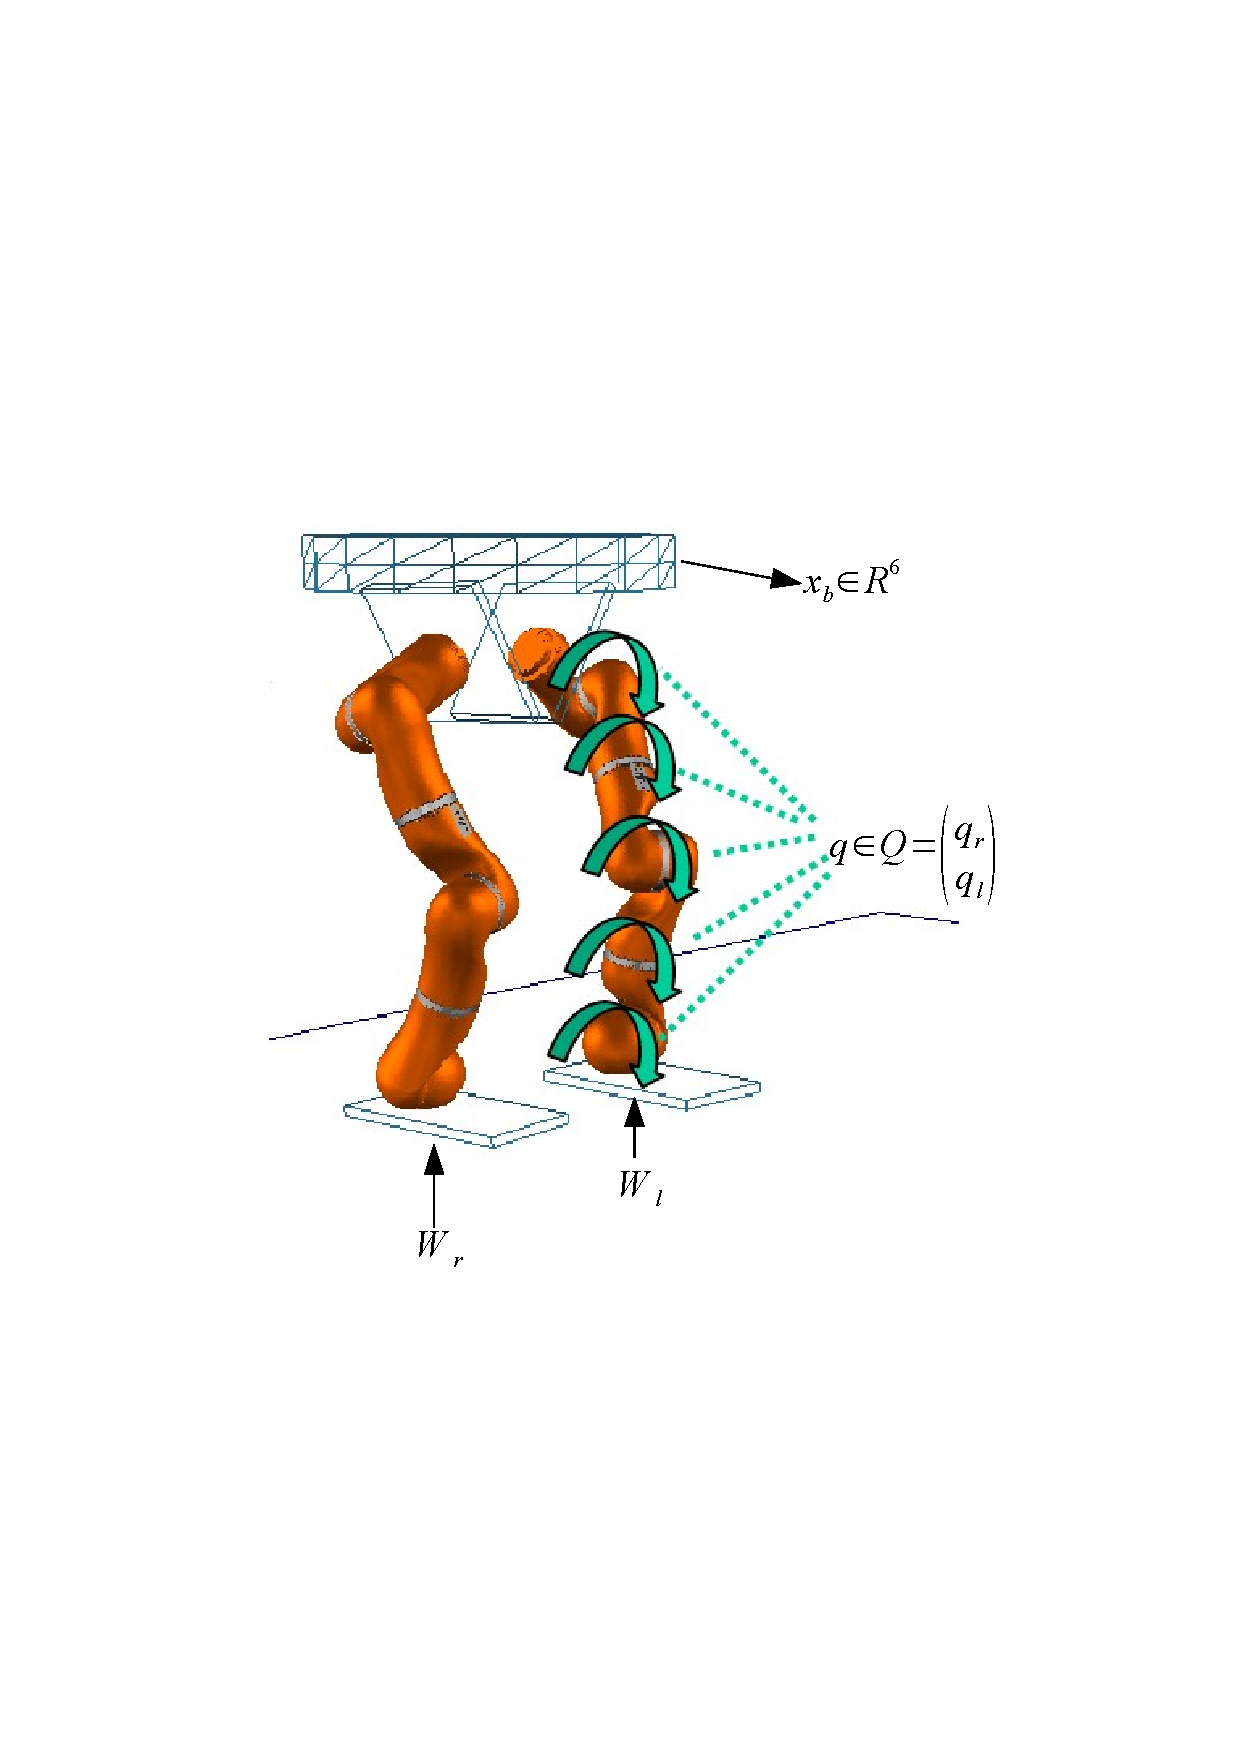
\includegraphics[trim= 10mm 80mm 10mm 80mm,scale=0.75]{Bilder/model_biped.pdf}
\caption{Simplified lower body model of biped}
\label{fig:biped_simplelow}
\end{center}
\end{figure}
Figure \ref{fig:biped_simplelow} shows a biped with two legs, which is connected to common base. The generalized coordinates of the robot legs is represneted by the vecotor of joint angles $q$. The vector $q$ consists of two subvectors $q_r,q_l$ that corresponds to angles of the joints in left and right legs respectively. Number of joints in a multi body system is the number of controllable degrees of freedom of the system. \emph{Q} is the configuration space of the biped. Configuration space represents the set of all valid configurations of the system. Each element of $q$ corresponds to the valid configuration of the system \cite[Chapter 2]{mur94}. $x_b$ represents the number of degrees of freedom of the base. A rigid body in space has six degrees of freedom as shown in Figure \ref{fig:rbody}.
%\begin{figure}[!htb]
\begin{figure}
\begin{center}
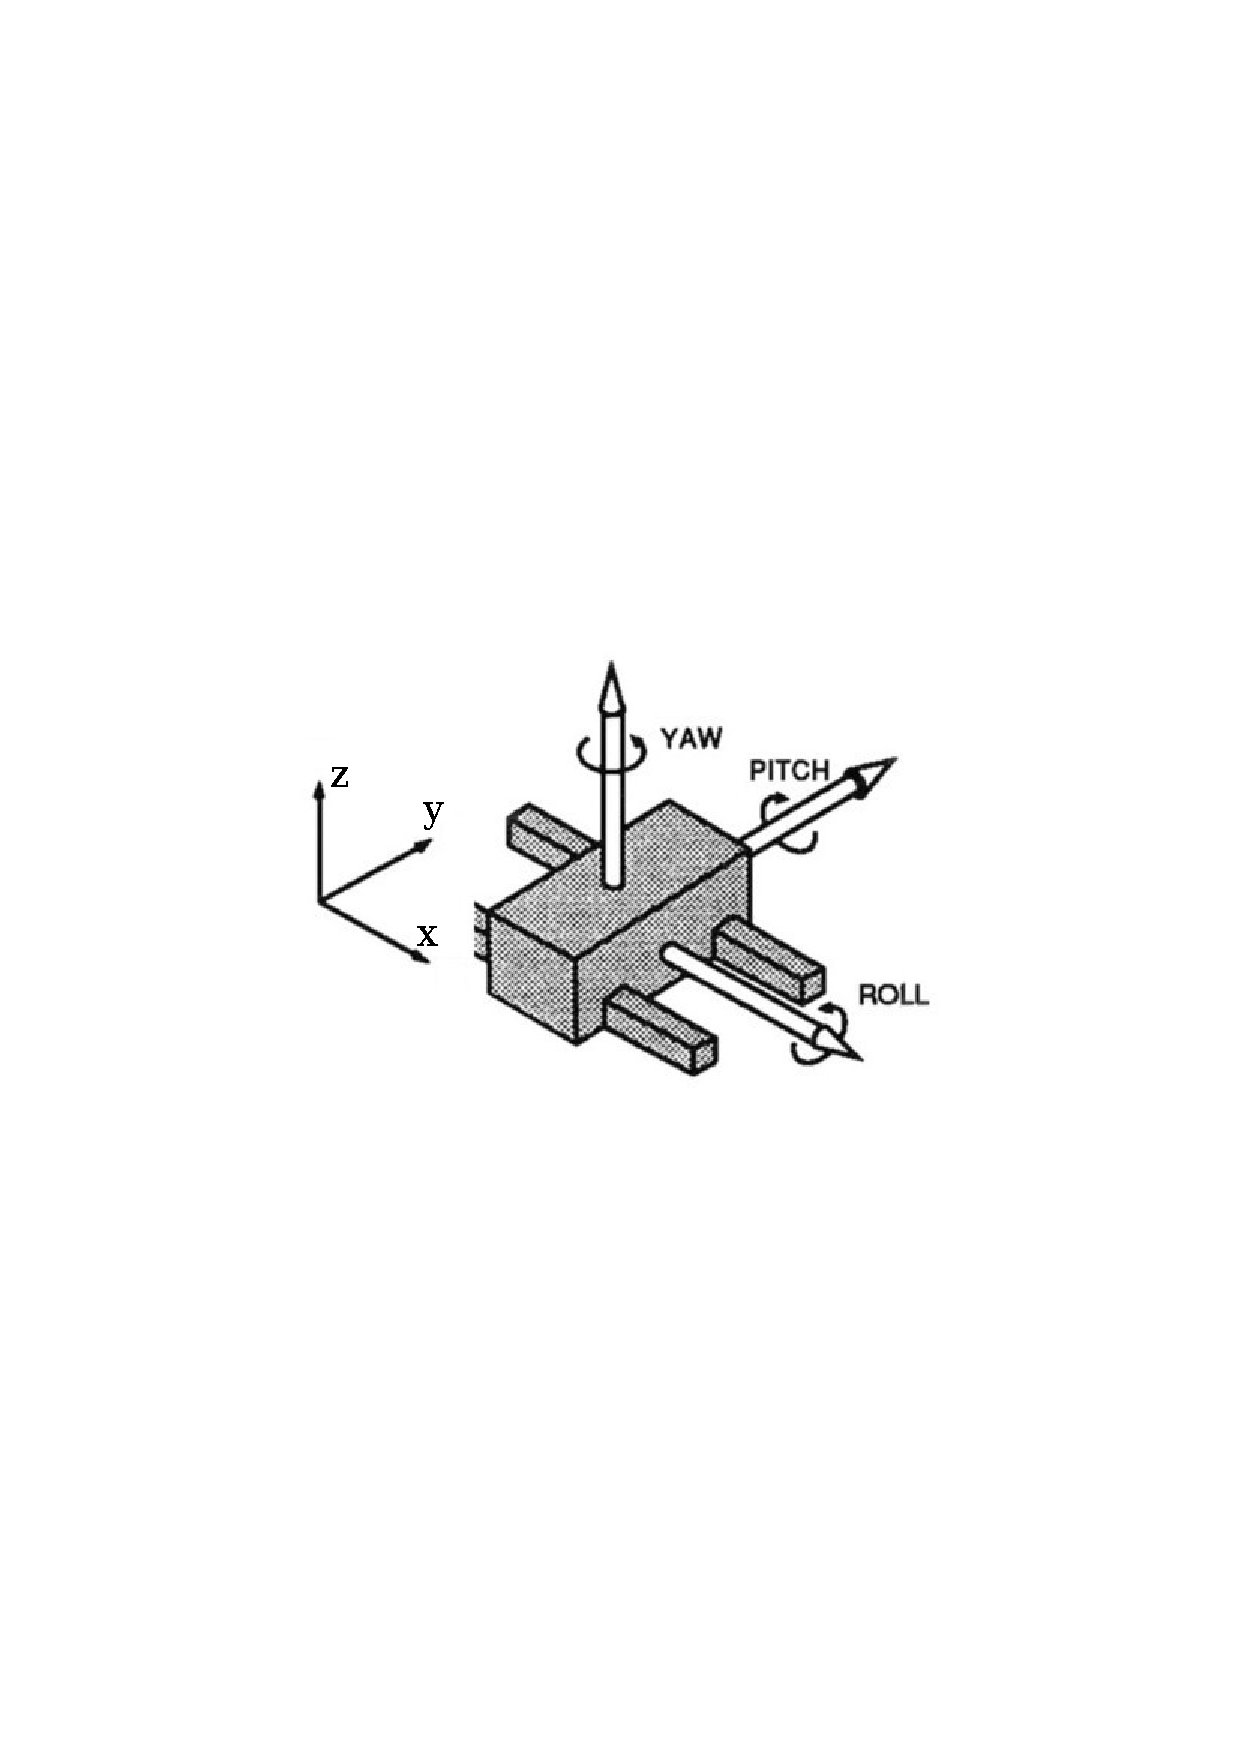
\includegraphics[trim= 30mm 100mm 10mm 120mm,scale=0.75]{Bilder/rbody_dof.pdf}
\caption[Degrees of freedom of a rigid body]{Degrees of freedom of a rigid body \footnotemark[1]}
\label{fig:rbody}
\end{center}
\end{figure}
The translational degrees of freedom of the rigid body in Figure \ref{fig:rbody} is \emph{x,y,z} and \emph{roll,pitch,yaw} are the rotational degrees of freedom which corresponds to rotation around \textbf{X,Y,Z} axes respectively. In biped, the base is a free rigid body which is unactuated. The base of the biped has all six degrees of freedom unless it is constrained to the surface as shown in Figure \ref{fig:biped_simplelow}. Since the base has all the six degrees of freedom it is called floating base. The equation of motion of a single rigid body(floating base) is given by Newton-Euler equation of motion in body coordinates \cite[Chapter 4]{mur94}. It is given by 
\footnotetext[1]{Image source:\url{http://www.cncexpo.com/Images/pitchyawroll.jpg}}
\begin{equation}
\label{eq:dyn_rig_bdy}
\begin{bmatrix}
mI_3 & \textbf{0}_3 \\ \textbf{0}_3 &\Im
\end{bmatrix}
\begin{bmatrix}
\dot{v}^b\\ \dot{\omega}^b
\end{bmatrix}
+ \begin{bmatrix}
\omega^b \times mv^b \\ 
\omega^b \times \Im w^b
\end{bmatrix}
= W^b,\\
\end{equation}
where \emph{m} is the mass of the rigid body, $\Im$ is the moment of inertia of the rigid body. $I_3$ represents the $3 \times 3$ identity matrix and $ \textbf{0}_3$ represents the  $3 \times 3$ zero matrix. $[\dot{v}^b,\dot{\omega}^b]$ are the translational velocity and angular velocity represented in body coordinate frame. $W^b$ is the \underline{body wrench}  applied to the center of mass of body. To be consistent with the multi body system dynamics formulation in Equation \ref{eq:dyn_mul_bdy} Newton Euler Equation \ref{eq:dyn_rig_bdy} is reformulated as
\begin{equation}
\label{eq:dyn_rig_bdy_sh}
M_x^b \ddot{x}_f^b + C_x^b\dot{x}_f^b+g_x^b = W^b,
\end{equation}
 where $x_f^b$ is a vector that represents six degrees of freedom of the rigid body, $\dot{x}_f^b$ represents the body velocity, $\ddot{x}_f^b$ represents the acceleration in body frame(i.e it represents the time derivative of body twist). $M_x^b$ represents the inertia matrix of the rigid body in body coordinates. $C_x^b$ is the matrix representing the Coriolis and centrifugal forces acting on the system in body coordinates. $g_x^b$ is the vector representing the gravitational forces acting on the body in body coordinates. $W^b$ is the external force applied to the center of mass of the body. \footnote[2]{Inertia, Coriolis and gravity are assumed to be given with respect to the body coordinate frame for the rest of the report}.

The equations of motion of the biped in Figure \ref{fig:biped_simplelow} is composed of equation of motion of the multi body system (For example legs) and equation of motion of single rigid body (For example the floating base). The composed equation of motion of the biped is \cite{ott09} 
\begin{equation} \label{eq:dyn_biped}
\begin{bmatrix}
M_x &M_{xq} \\ M_{qx} &M_q
\end{bmatrix}
\begin{bmatrix}
\ddot{x}_f \\ \ddot{q}
\end{bmatrix}
+
\begin{bmatrix}
C_x &C_{xq} \\ C_{qx} &C_q
\end{bmatrix}
\begin{bmatrix}
\dot{x}_f \\ \dot{q}
\end{bmatrix}
+
\begin{bmatrix}
g_x \\ g_q
\end{bmatrix}
=
\begin{bmatrix}
0 \\ \tau
\end{bmatrix}
+ (J_r^b)^T W_r^b + (J_l^b)^T W_l^b,
\end{equation}
where the terms with subscript $x$ are the parameters of floating  base, the terms with subscript $q$ are the parameters of the multi body system(legs) and the terms with subscript $xq, qx$ are the coupling terms that connects the dynamics of the floating base with dynamics of the multibody system.

Equation \ref{eq:dyn_biped} can be written in a simplified form as
\begin{equation} \label{eq:dyn_sbiped}
M(y)\ddot{y} + C(y,\dot{y})\dot{y} + g(y) = \tau + J^T W_{ext},
\end{equation}
where $y = \begin{bmatrix} x_f \\ q \end{bmatrix}$ is the state variables of the biped, and $W_{ext}$ is the external wrench acting on the system (For example $W_l,W_r$ in \ref{eq:dyn_biped} are the external wrenches acting on the biped).
\begin{figure}
\begin{center}
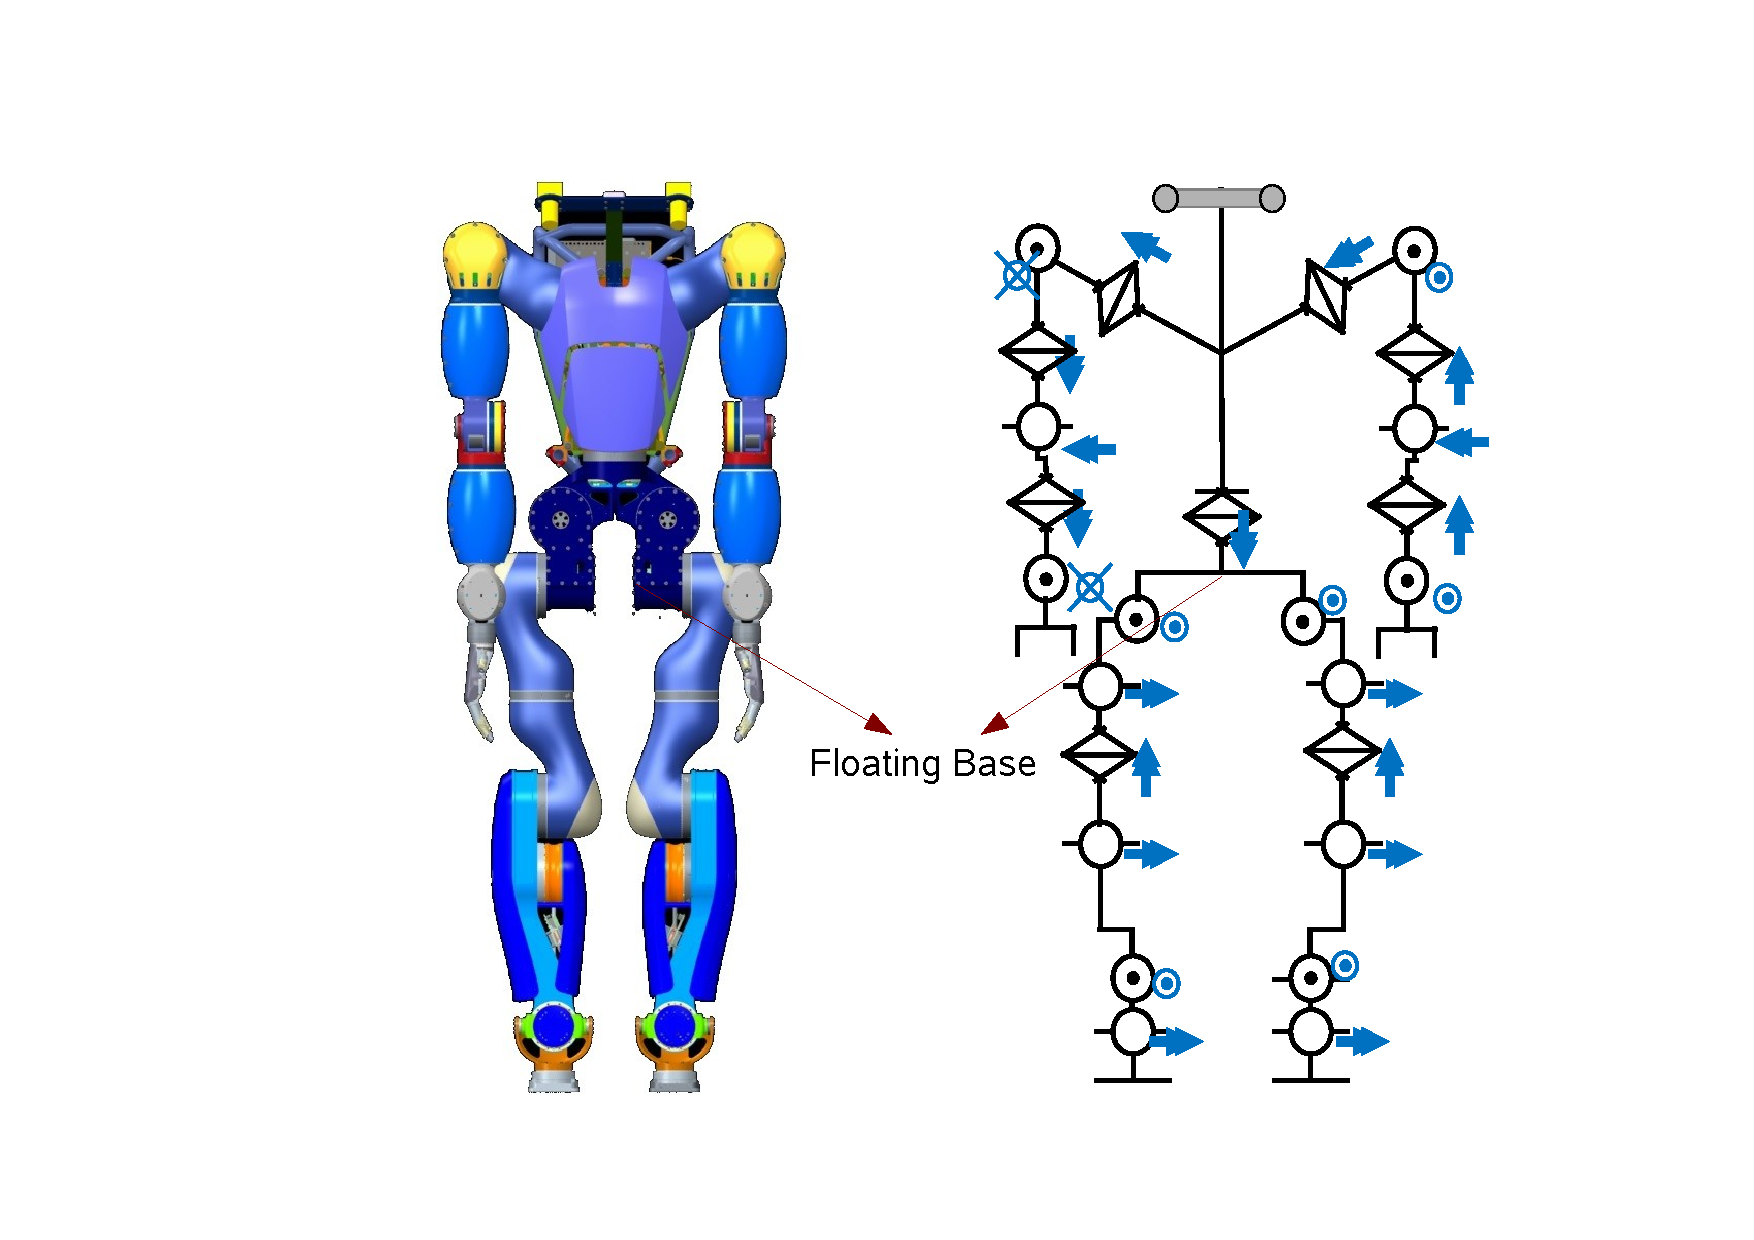
\includegraphics[trim= 70mm 10mm 40mm 10mm,clip,scale=0.7]{Bilder/TORO_kinematic.pdf}
\caption{Kinematic chain of \emph{Toro} \underline{Explain the joints symbols}}
\label{fig:toro_kin}
\end{center}
\end{figure}
\paragraph{Toro}
\emph{Toro} is modelled as floating base dynamic model. \emph{Toro} is made up of 25 rotary joints that are actuated by electrical motors. It can be seen from Figure \ref{fig:toro_kin} that floating base acts as the root of the kinematic chain. Legs and torso branches out of the floating base. Equation of motion for \emph{Toro} can be formulated in similar fashion as biped Equation \ref{eq:dyn_sbiped}, where the dynamics of the upper body is also combined to it. The forward dynamics of \emph{Toro} 
\begin{equation}
	\label{eq:motion}
	\begin{split}
	\ddot{y} = M(y)^{-1}(&-C(y,\dot{y})\dot{y} - g(y) + J_r(y)^{T}W_{r} +J_l(y)^{T}W_{l} + \tau) \\
	\text{where,}\\ y &=
	\begin{bmatrix}
	 x_f \\ q 
	\end{bmatrix} \in \Re ^{31} \\
	x_f &= [p,\theta]^T \in \Re ^6 \\
	q &= [q_{1},q_{2},\ldots , q_{25}]^T \in \Re ^{25}\\
	\end{split}
\end{equation}
\emph{q} is a vector of joint variables given in generalized coordinates. $x_{f}=[p,\theta]^{T}$ is a vector of position and orientation defined with respect to spatial frame. $p=[p_x,p_y,p_z]$ is a vector representing  the position of origin of floating base with respect to spatial frame and $\theta=[\theta_{x},\theta_{y},\theta_{z}]$ is a vector of \underline{Euler angles}  that describes the rotation of floating base frame with respect to spatial frame. $q \in \Re^{25}$ is the vector of joint angles. $\dot{y}=[V^{b},\dot{q}]^T \in \Re^{31}$ is the vector of generalized velocities. $V^b= [v^b,\omega^b]^T \in \Re^{6}$ is the body velocity, it is defined in \ref{eq:body_vel}. $\dot{q} \in \Re^{25}$ is the vector of joint velocities. $\ddot{y}\in \Re^{31}$ is the vector of generalized accelerations. $M(y)\in \Re^{31 \times 31}$ is the inertia matrix, $C(y,\dot{y})\in \Re^{31 \times 31}$ is the matrix accounting for centrifugal and Coriolis forces. $g(y) \in \Re^{31}$ is the gravity vector. $\tau \in \Re^{31}$ is the vector of actuating torques acting on the robot, where the first six components are zero because those degrees of freedom corresponding to $x_f$ are not actuated. $J_r(y)^{T},J_l(y)^{T} \in \Re^{31 \times 6}$ represents the body Jacobian that transforms the wrenches $W_r,W_l \in \Re^{6}$ applied in the right and left foot to generalized forces acting on the robot.

Integrating the forward dynamics Equation \ref{eq:motion} once gives the velocity of all the bodies in the system and integrating it twice gives the position or orientation of the system. $$ acc = \dfdx{^2pos}{t}, vel = \dfdx{pos}{t} $$ 
\subsection{State space representation:}
The multi body system would be modelled with position(\emph{pos}) and velocity(\emph{vel}) as the state variables which leads to following form 
\begin{equation}
\label{eq:newton_motion}
 \begin{bmatrix}
\dot{pos} \\ \dot{vel}
\end{bmatrix}
= \begin{bmatrix}
vel \\ acc
\end{bmatrix}
\end{equation}
acceleration(\emph{acc}) is given by the forward dynamics of the system.

The equations of motion in Equation \ref{eq:motion} should be formulated in state space form of non linear systems as given in \ref{eqn:nl_sys}.
\begin{comment}
General state space representation of a non linear system
\begin{equation}
\label{eq:dyn_nl}
	\begin{split}
	\dot{x} = f(x,u)\\
	y = h(x,u)
	\end{split}
\end{equation}
where, $x \in \Re^{n}$ is the vector representing the states of the system. $u \in \Re^{p}$ is the vector of inputs acting on the system. $y \in \Re^{m}$ is the vector of outputs of the system.\\
\end{comment}
The velocity of the free floating base of the robot is modelled as body velocity $V_f^b$ which is given as,
\begin{equation}
\label{eq:body_vel}
V^b =
\begin{bmatrix}
v^b \\ \omega^b
\end{bmatrix}
= \begin{bmatrix}
R^T \dot{p} \\ (R^T \dot{R})^\vee
\end{bmatrix}
\end{equation}
$\vee$ operator denotes represents the extraction of 3 dimensional vector from the symmetric matrix[Appendix \ref{sec:avel_trfm}]
$\dot{p}$ is the time rate of change of the position of the body. \emph{R} is the rotation matrix which describes the rotation of rigid body with respect to \underline{spatial frame}. It is possible to reformulate the translational velocity of the above equation in first order \underline{ODE(Ordinary Differential Equation)}. It is not straight forward to obtain the time rate of change of Euler angles $\dot{\theta}$. There exists a transformation between the $\dot{\theta}$ and angular velocity $\omega^b$.
\begin{equation}
\label{eq:transfo_angvel}
\begin{split}
\omega^b = T(\theta)\dot{\theta}
\end{split}
\end{equation}
$T(\theta)$ is the transformation matrix [Appendix \ref{sec:avel_trfm}]. 

The state space representation of the equation of motions of \emph{Toro} can be obtained by substituting Equations \ref{eq:body_vel}, \ref{eq:transfo_angvel} and \ref{eq:motion} in Equation \ref{eq:newton_motion}

\begin{equation}
\label{eq:toro}
	\dot{x} = 
	\begin{bmatrix}
	\dot{p} \\ \dot{\theta} \\ \dot{q} \\ \ddot{y}
	\end{bmatrix}
	=
	\begin{bmatrix}
	R v^b\\	
	T(\theta)^{-1} \omega_f^b \\
	\dot{q}\\
	M(y)^{-1}(-C(y,\dot{y})\dot{y} -g(y) +  J_r(y)^{T}W_{r} +J_l(y)^{T}W_{l} + \tau)	
	\end{bmatrix}
	\\
	\end{equation}	
\begin{itemize}
\item $$ y = \begin{bmatrix} p \\ \theta \\ q \end{bmatrix} = \begin{bmatrix} x_f \\ q \end{bmatrix}, \dot{y} = \begin{bmatrix} V^b \\ \dot{q}\end{bmatrix}, x = \begin{bmatrix}y \\ \dot{y}\end{bmatrix} $$  $x_f,q$ are the parameters of the floating base and joints as described in \ref{eq:motion}. $V^b$ is the body velocity as defined in \ref{eq:body_vel} and $\dot{q}$ is the velocities of the joints of the robot. \emph{x} is the vector of system states.
\item $T(\theta_{f})$ is the matrix that transforms the angular velocity $\omega_{f}^{b}$ to the time derivative of Euler angles $\dot{\theta}_{f}$. i.e $\omega_{f}^{b}=T(\theta_{f}) \dot{\theta}_{f}$. 
\item R is the rotation matrix which describes the rotation of floating base with respect to spatial frame. $ R = R_x(\theta_x) R_y(\theta_y) R_z(\theta_z)$
\end{itemize}

\section{Prediction step}
The prediction equations of EKF are given in Equation \ref{eq:ekf_predict}. For the sake of simplicity we assume the process noise acting on the model is uncorrelated. i.e The noise acting on each state is independent $$W_k = I_{n}$$. \emph{n} is the number of states. Substituting the value of $W_k$ in Equation \ref{eq:ekf_predict}
\begin{equation}
\label{eq:predict}
\begin{split}
\hat{x}_{k+1}^- &= f(\hat{x}_{k},u_{k+1},0)\\
P_{k+1}^- &= A_kP_{k}A_k^T + Q_{k}\\
\end{split}
\end{equation}
The model is discretized for the implementation of EKF. Since the time step for integration is very small $\Delta t = 1ms$ forward Euler discretization method is used to discretize the continuous time model in \ref{eq:toro}.
\begin{equation}
\label{eq:toro_dis}
	\begin{bmatrix}
	\hat{p}_{k+1}^- \\ \hat{\theta}_{k+1}^- \\ \hat{q}_{k+1}^- \\ \hat{\dot{y}}_{k+1}^-
	\end{bmatrix}
	 =   
	 \begin{bmatrix}
	 \hat{p}_k \\ \hat{\theta}_k \\ \hat{q}_k \\ \hat{\dot{y}}_{k}
	\end{bmatrix}	  
	+ \Delta t f(\hat{x}_k,u_{k+1}) \\
\end{equation}
$$ f(\hat{x}_k,u_{k+1}) = 
	\begin{bmatrix}
	R v^b_k\\	
	T(\hat{\theta}_k)^{-1} \omega_k^b\\
	\dot{q_k}\\
	M(\hat{y}_{k})^{-1}(-C(\hat{y}_{k},\hat{\dot{y}}_{k})\hat{\dot{y}}_{k} -g(\hat{y}_{k}) +  J_r(\hat{y}_{k})^{T}W_{r,k+1} +J_l(\hat{y}_{k})^{T}W_{l,k+1} + \tau_{k+1})	
	\end{bmatrix} $$
$\hat{x}(t_k) = \hat{x}(k \Delta t) = \hat{x}_k$ represents the state x at \emph{kth} sampling instant. $\hat{x}_{k+1} = \hat{x}(k \Delta t + \Delta t)$ represents the state of the system at the next sampling instant. $u_{k+1}$ is the input at sampling instant $k+1$. It is assumed that the value of the input remains constant in the interval between two sampling instant. This assumption is valid because of the zero order hold mechanism in sensor circuitry.

Equation \ref{eq:toro_dis} is used to predict the state $\hat{x}_k$ in Equation \ref{eq:predict}. For the computation of state covariance matrix $P_k^-$ in Equation \ref{eq:predict}, the \underline{Jacobian Matrix} is computed for Equation \ref{eq:toro_dis}. \underline{The Jacobian} computation of the different parts of the equation is follows,
From Equation \ref{eq:toro_dis}
\begin{enumerate}
\item $ \hat{p}_{k+1}^- = \hat{p}_k + \Delta t Rv_b$, $ \hat{p}_k = [\hat{p}_{x,k},\hat{p}_{y,k},\hat{p}_{z,k}]$
\begin{equation}
\label{eq:dpdx}
\dfdx{\hat{p}_{j,k+1}^-}{x} = \left(\dfdx{\hat{p}_{j,k+1}^-}{x_{1}}, \dfdx{\hat{p}_{j,k+1}^-}{x_{2}}, \cdots , \dfdx{\hat{p}_{j,k+1}^-}{x_{62}}\right) \in \Re^{3 \times 62}
\end{equation}
\[
 \dfdx{\hat{p}_{k+1}^-}{x_{i}} =  \left\lbrace
  \!\begin{aligned}
   &e_i & \text{if }(i=j)\\
   &\Delta t \dfdx{R}{x_i}v_b & \text{if }(3 < i \leq 6)\\
   &\textbf{0}_{3 \times 1} &\text{if}(6 < i \leq 31) \text{ or } (35 < i \leq 62) \\
   &col(R,i-31) & \text{if } 31 < i \leq 34 \\
  \end{aligned} \right.
\]
\begin{itemize}
\item \emph{j} in the subscript represents the row dimension and  \emph{i} represents the column dimension of the matrix in Equation \ref{eq:dpdx}
\item $col(X,i)$ - represents the \emph{ith} column of matrix $X$.
\item $\dfdx{R}{x_i}$ is the partial derivative of \emph{R} with respect to the state $\hat{x}_k$ (i.e euler angles [Appendix \ref{sec:rot_mat}]), $e_i$ is the unit vectors in direction of coordinate axis and  $\textbf{0}_{3 \times 1}$ is the zero vector of dimensions $3 \times 1$ [Appendix \ref{sec:symbols}].
\end{itemize}

\item $\hat{\theta}_{k+1}^- = \hat{\theta}_k + \Delta t T(\hat{\theta}_k)^{-1} \omega_k^b$
\begin{equation}
\label{eq:dthetadx}
\dfdx{\hat{\theta}_{j,k+1}^-}{x} = \left(\dfdx{\hat{\theta}_{j,k+1}^-}{x_{1}}, \dfdx{\hat{\theta}_{j,k+1}^-}{x_{2}}, \cdots , \dfdx{\hat{\theta}_{j,k+1}^-}{x_{62}}\right) \in \Re^{3 \times 62}
\end{equation}
\[
 \dfdx{\hat{\theta}_{k+1}^-}{x_{i}} = \left\lbrace
  \!\begin{aligned}
   &\textbf{0}_{3 \times 1} &\text{if}(0 < i \leq 3) \text{ or }(6 < i \leq 31) \text{ or } (35 < i \leq 62) \\
   &e_{i-3} + \Delta t \dfdx{T(\hat{\theta}_k^-)^{-1}}{x_i}\omega_k^b & \text{if}3< \text{i} \leq 6 \\
   &col(T(\hat{\theta}_k^-)^{-1},i-34) & \text{if } 31 < i \leq 34 \\
  \end{aligned} \right.
\]
\begin{itemize}
\item $\dfdx{T(\theta_k^-)^{-1}}{x_i}$ is the partial derivative of inverse of transformation matrix with respect to state [Appendix \ref{sec:avel_trfm}] 
\end{itemize}

\item $\hat{q}_{k+1}^- = \hat{q}_k + \Delta t \dot{q}_k $
\begin{equation}
\label{eq:dqdx}
\dfdx{\hat{q}_{k+1}^-}{x} = \left(\dfdx{\hat{q}_{k+1}^-}{x_{1}}, \dfdx{\hat{q}_{k+1}^-}{x_{2}}, \cdots , \dfdx{\hat{q}_{k+1}^-}{x_{62}}\right) \in \Re^{25 \times 62}
\end{equation}
\[
\dfdx{\hat{q}_{k+1}^-}{x_{i}} = 
	\begin{cases}
	l_{25,i} & \text{if } (6 < i \leq 31) \text{ or } (38 < i \leq 62) \\
	0 & \text{otherwise}   \\
	\end{cases}
\]
\begin{itemize}
\item $l_{25,i}$ is a column vector of length 25 with 1 in the \emph{ith} position and zeros in other position [Appendix \ref{sec:symbols}].
\end{itemize}
\item $\hat{\dot{y}}_{k+1}^- = \hat{\dot{y}}_{k}+ \Delta t \Lambda $
$$\Lambda = M(\hat{y}_{k})^{-1}(-C(\hat{y}_{k},\hat{\dot{y}}_{k})\hat{\dot{y}}_{k} - g(\hat{y}_{k}) + J_r(\hat{y}_{k})^{T}W_{r,k+1} +J_l(\hat{y}_{k})^{T}W_{l,k+1} + \tau_{k+1})$$
 \begin{equation}
 \label{eq:dydx}
\dfdx{\hat{\dot{y}}_{k+1}^-}{x} = \left(\dfdx{\hat{\dot{y}}_{k+1}^-}{x_{1}}, \dfdx{\hat{\dot{y}}_{k+1}^-}{x_{2}}, \cdots , \dfdx{\hat{\dot{y}}_{k+1}^-}{x_{62}}\right) \in \Re^{31 \times 62}
\end{equation}
where,
\[
\dfdx{\hat{\dot{y}}_{k+1}^-}{x_{i}} = 
\left\{ 
\!\begin{aligned}
	& \left. \!\begin{aligned}
	-M_k^{-1}\dfdx{M_k}{x_{i}}\Lambda + &M_k^{-1}\left(-\dfdx{C_k}{x_{i}}\hat{\dot{y}}_{k} -\dfdx{g_k}{x_{i}}        + \left(\dfdx{J_{r,k}^{b}}{x_{i}}\right)^{T}W_{r,k+1}\right) \\
	& + M_k^{-1}\left(\dfdx{J_{l,k}^{b}}{x_{i}}\right)^{T}W_{l,k+1}
	\end{aligned} \right\}& \text{if } 0 < i \leq 31 \\
&l_{31,(i-31)}-M_k^{-1}\dfdx{M_k}{x_{i}}\Lambda + M_k^{-1}\left(-\dfdx{C_k}{x_{i}}\hat{\dot{y}}_{k}- col(C_k,i-31)\right) & \text{if } i < 31  \\
\end{aligned}
\right.
\]
\begin{itemize}
\item $M_k= M(\hat{y}_{k}),C_k=C(\hat{y}_{k},\hat{\dot{y}}_k),J_{r,k}=J_r(\hat{y}_{k}),J_{l,k}=J_l(\hat{y}_{k})$
\end{itemize}
The system matrix $A_k$ in Equation \ref{eq:predict} is formulated by combining Equations \ref{eq:dpdx},\ref{eq:dthetadx},\ref{eq:dqdx} and \ref{eq:dydx}
\begin{equation}
\label{eq:sys_mat}
A_k = \left(
\begin{aligned}
\dfdx{\hat{p}_{k+1}^-}{x} \\
\dfdx{\hat{\theta}_{k+1}^-}{x} \\
\dfdx{\hat{q}_{k+1}^-}{x}\\
\dfdx{\hat{\dot{y}}_{k+1}^-}{x}
\end{aligned} \right)
\in \Re^{62 \times 62}
\end{equation}
Substituting Equations \ref{eq:toro_dis} and \ref{eq:sys_mat} in \ref{eq:predict} and substituting the values of process covariance $Q_k$ completes the prediction stage of EKF.

\section{Update step}
The update equation of the EKF is given in Equation \ref{eq:ekf_correct}. The measurement equation of the system is given by $$\hat{y}_{k+1} = h(\hat{x}_{k+1}^-,u_{k+1},0)$$.For the sake of simplicity let us assume the measurement of noise are independent. $$V_k = I_3$$. Substituting the assumption in \ref{eq:ekf_correct}
\begin{equation}
\label{eq:correct}
\begin{split}
K_{k+1} &= P_{k+1}^-\hat{H}_{k+1}^{T-}(\hat{H}_{k+1}^-P_{k+1}^-\hat{H}_{k+1}^{T-} + R_{k+1})^{-1}\\
\hat{x}_{k+1} &= \hat{x}_{k+1}^- + K_{k+1}(y_{k+1}-\hat{y}_{k+1})\\
P_{k+1} &= (I- K_{k+1}\hat{H}_{k+1}^-)P_{k+1}^-
\end{split}
\end{equation}
The measurements of \emph{Toro} are Cartesian accelerations($acc^b$) of the hip measured by accelerometer($IMU_{acc}$), angular velocity($\omega^b$) of the hip measured by the gyroscope($IMU_{gyro}$), joint angles($q_j$) and joint velocities($\dot{q_j}$) measured by joint encoders.
\begin{equation}
    \label{eq:y_sens}
     y_{sens} = \begin{bmatrix} acc^b \\ \omega^b \\ q_j \\ \dot{q}_j \end{bmatrix} 
\end{equation}
\begin{itemize}
    \item The simplified model of $IMU_{acc}$ is $$ acc^b= \begin{bmatrix} acc^b_x \\ acc^b_y \\ acc^b_z \end{bmatrix} =  \begin{bmatrix}\ddot{p}_x^b \\ \ddot{p}_y^b \\ \ddot{p}_z^b \end{bmatrix} - R^T \begin{bmatrix}0 \\0 \\-9.81 \end{bmatrix}$$ \emph{R} is the rotational matrix that transforms a vector in body coordinate frame to spatial frame.
    \item $\ddot{p}^b$ is computed from the forward dynamic equation \ref{eq:motion} using the predicted values of the state
    \item $\omega_{f}^{b} $ is the vector of angular rates of the hip(floating base) measured by gyroscope. The measurements are in the frame attached to the hip. 
\end{itemize}
\begin{figure}
    \begin{center}
    %trim option's parameter order: left bottom right top
    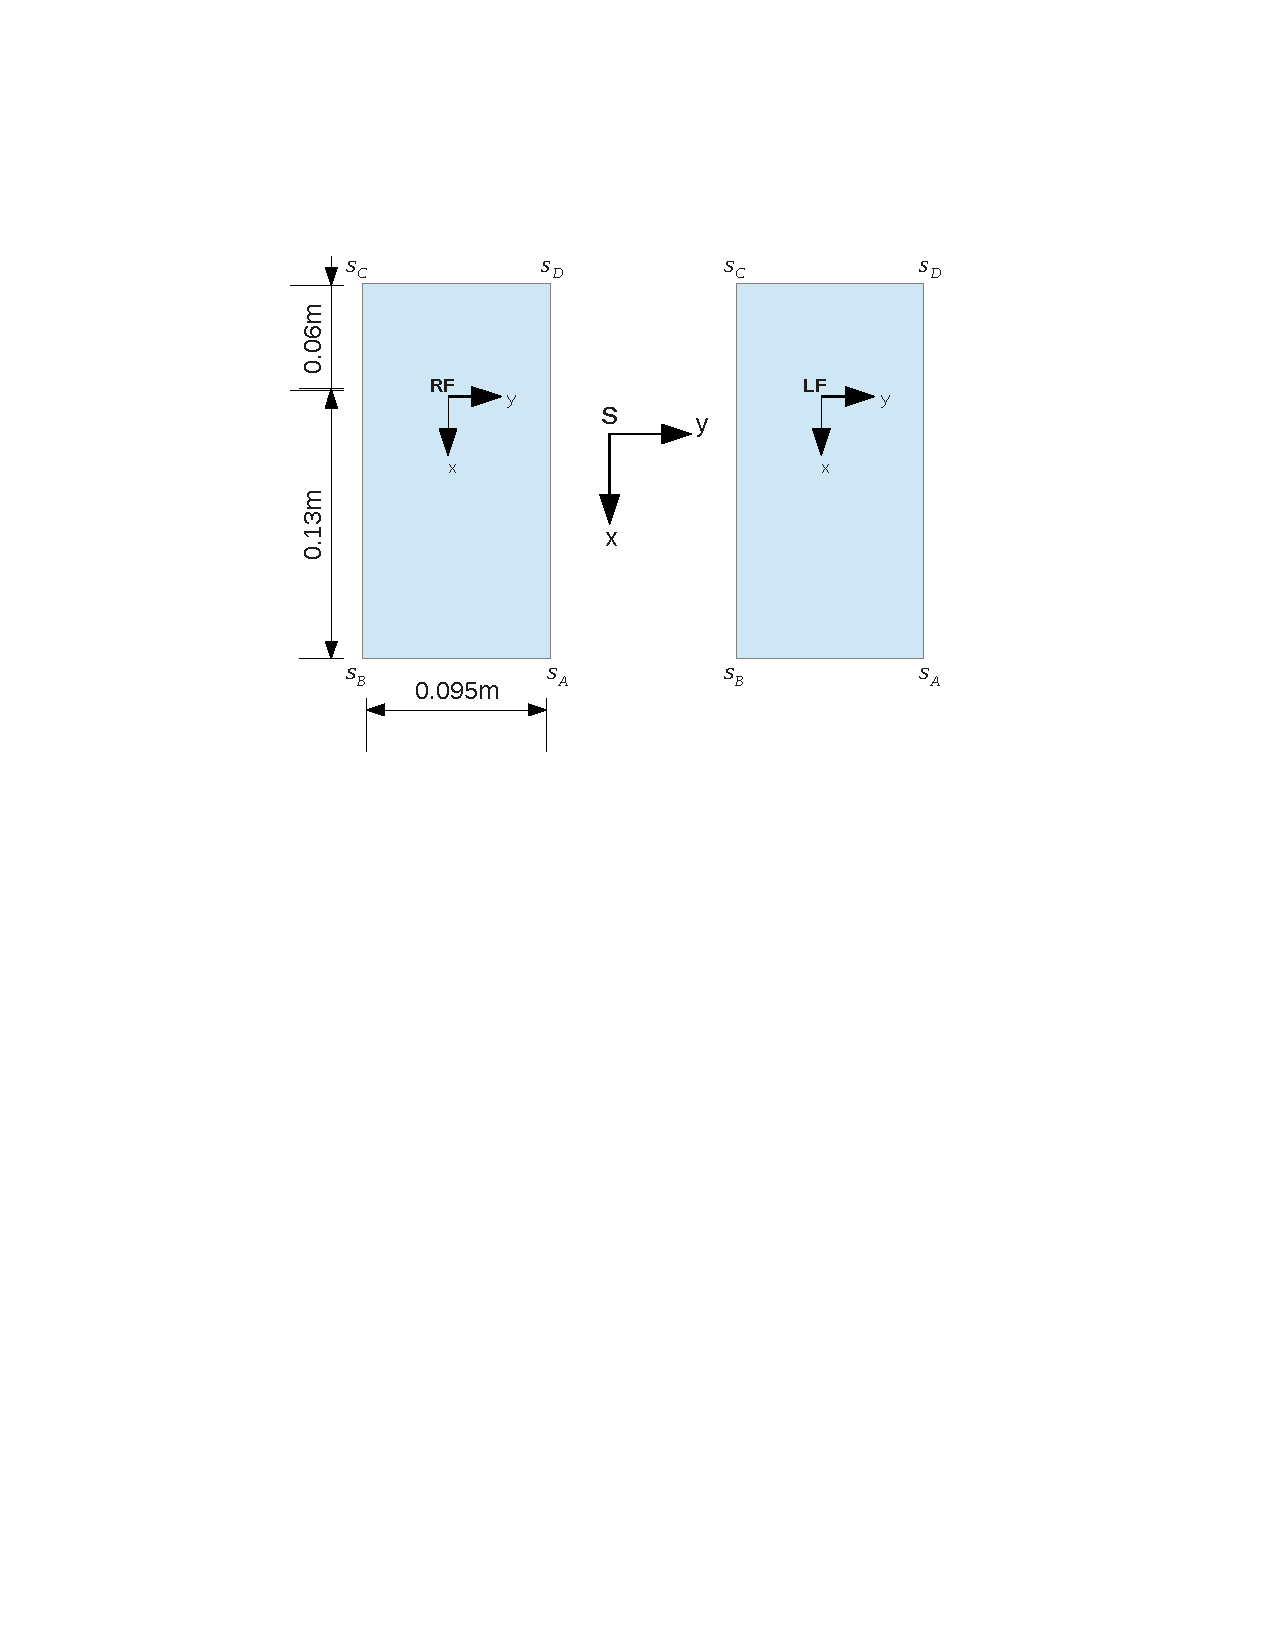
\includegraphics[trim= 20mm 150mm 20mm 50mm,scale=0.80]{Bilder/foot_topview.pdf}
    \caption{Toro feet viewed from top}
    \label{fig:biped_feet}
    \end{center}
\end{figure}
Along with the sensor measurements kinematic constraints are also considered as mesurement. When a foot is in contact with the ground the velocity of the foot is zero. Figure \ref{fig:biped_feet} shows the contact points considered for measurements. The corner points of each foot are measured with respect to spatial frame \emph{S} as shown in Figure \ref{fig:biped_feet} before starting the experiment and they are assumed to be constant throughout the experiment. The contact points of the robot does not change throughout the experiment, since we are considering the case where the robot is tilting around one edge of the foot. 
\begin{equation}
    \label{eq:y_kin}
    \begin{split}
    y_{kin} &=
    \begin{bmatrix}
    p_{contact} \\ V_{contact}
    \end{bmatrix}\\
    p_{contact} &= \begin{bmatrix}p_{RF}\\ p_{LF}\end{bmatrix}\\
     V_{contact} &= \begin{bmatrix} V_{RF}^b \\ V_{LF}^b \end{bmatrix} = \begin{bmatrix} J_r(\hat{y})^T \hat{\dot{y}} \\ J_l(\hat{y})^T\hat{\dot{y}} \end{bmatrix}
    \end{split}
\end{equation}
\begin{itemize}
\item $p_{RF},p_{LF}$ are the vectors of contact points in right foot and left foot defined with respect to spatial frame.
\item $J_r(y), J_l(y)$ are the Jacobian of right and left foot that relates the joint velocity to the velocity of right and left foot respectively. \underline{[Appendix Define Body Jacobian]}
\end{itemize}
\begin{equation}
    \begin{split}
    p_{RF} &= \begin{bmatrix} p_{A,RF}\\ p_{B,RF}\\ p_{C,RF}\\ p_{D,RF}\end{bmatrix}= \begin{bmatrix} {H}_{RF}p_{A}\\  {H}_{RF}p_{B}\\  {H}_{RF}p_{C}\\  {H}_{RF}p_{D}\end{bmatrix} \\
    p_{LF} &= \begin{bmatrix} p_{A,LF}\\ p_{B,LF}\\ p_{C,LF}\\ p_{D,LF}\end{bmatrix}= \begin{bmatrix} {H}_{LF}p_{A}\\  {H}_{LF}p_{B}\\  {H}_{LF}p_{C}\\  {H}_{LF}p_{D}\end{bmatrix} \\
    \end{split}
\end{equation}
\begin{itemize}
\item $\hat{H}_{RF},\hat{H}_{LF}$ are the homogeneous transformation matrices of the right and left foot [Appendix \ref{sec:htm}]
\item In Figure \ref{fig:biped_feet} $p_A,p_B,p_C,p_D$ are the corner points defined with respect to respective foot frame \emph{RF,LF}.
\end{itemize}
The full measurement equations of is obtained combining Equations \ref{eq:y_sens} and \ref{eq:y_kin} 
\begin{equation}
    \label{eq:y_msr}
    y_{k+1} = \begin{bmatrix} y_{sens,k+1} \\ y_{kin,k+1} \end{bmatrix}
\end{equation}
The measurement sensitivity matrix can be computed by taking the parial derivative of the measurement equation \ref{eq:y_msr} with respect to system states \emph{x}.
\begin{enumerate}
\item $\hat{acc}^b_{k+1} = \ddot{p}_{k+1}-\hat{R}^T\begin{bmatrix} 0 \\ 0 \\ -9,81 \end{bmatrix}$
\begin{equation}
    \label{eq:dacc_msrdx}
    \dfdx{\hat{acc}_{k+1}^{b-}}{x} = \dfdx{\hat{\ddot{p}}_{k+1}^{b-}}{x} + \dfdx{\hat{R}^{T-}_{k+1}}{x}\begin{bmatrix} 0 \\ 0 \\ -9,81 \end{bmatrix}  \in \Re^{3 \times 62}
\end{equation}
\begin{itemize}
    \item $\dfdx{\hat{\ddot{p}}_{k+1}^b}{x}$ is partial derivative of acceleration of body with respect to states of the system. It is computed by substituting $\hat{x}_{k+1}^-$ for $\hat{x}_k$ in Equation \ref{eq:dydx} and then subtracting  $l_{31,i-31}$ for the case \emph{i > 31}. The first three rows of the resulting matrix is the partial derivative of acceleration with respect to states.
    \item $\dfdx{\hat{R}^T_{k+1}}{x}$ is partial derivative of Rotation matrix with respect to system state.[Appendix \ref{sec:rot_mat}]
\end{itemize}

\item $\hat{\omega}^{b-}_{k+1}$
\begin{equation}
    \label{eq:dw_msrdx} 
    \dfdx{\hat{\omega}^{b-}_{k+1}}{x} = \left(\dfdx{\hat{\omega}^{b-}_{k+1}}{x_{1}}, \dfdx{\hat{\omega}^{b-}_{k+1}}{x_{2}}, \cdots , \dfdx{\hat{\omega}^{b-}_{k+1}}{x_{62}}\right) \in \Re^{3 \times 62}
\end{equation}
\[ \dfdx{\hat{\omega}^{b-}_{k+1}}{x} = 
    \begin{cases}
    l_{3,34-i} & \text{if } 34 < i \leq 37 \\
    \textbf{0}_{3,1} &\text{otherwise}
    \end{cases}
 \]  
 
\item $\hat{q}_{k+1}^-$
\begin{equation}
\label{eq:dq_msrdx}
\dfdx{\hat{q}_{k+1}^-}{x} = \left(\dfdx{\hat{q}_{k+1}^-}{x_{1}}, \dfdx{\hat{q}_{k+1}^-}{x_{2}}, \cdots , \dfdx{\hat{q}_{k+1}^-}{x_{62}}\right) \in \Re^{25 \times 62}
\end{equation}
 \[
 \dfdx{\hat{q}_{k+1}^-}{x_{i}} =
 \begin{cases}
 1 & \text{if } 7 \leq i \leq 31 \\
 0 & \text{otherwise}
 \end{cases}
 \]

\item  $\hat{\dot{q}}_{k+1}^-$
\begin{equation}
 \label{eq:ddq_msrdx}
\dfdx{\hat{\dot{q}}_{k+1}^-}{x} = \left(\dfdx{\hat{\dot{q}}_{k+1}^-}{x_{1}}, \dfdx{\hat{\dot{q}}_{k+1}^-}{x_{2}}, \cdots , \dfdx{\hat{\dot{q}}_{k+1}^-}{x_{62}}\right) \in \Re^{25 \times 62}
\end{equation}
  \[
 \dfdx{\hat{\dot{q}}_{k+1}^-}{x_{i}} =
 \begin{cases}
 1 & \text{if } 37 < i \leq 62 \\
 0 & \text{otherwise}
 \end{cases}
 \]
 \item $\hat{p}_{RF,k+1}^- = \hat{H}_{RF,k+1}^- p = \begin{bmatrix} \hat{H}_{RF,k+1}^- p_{A}\\ \hat{H}_{RF,k+1}^- p_{B}\\ \hat{H}_{RF,k+1}^- p_{C}\\ \hat{H}_{RF,k+1}^- p_{D}\end{bmatrix}$
\begin{equation}
    \label{eq:dpr_msrdx}
    \begin{split}
    &\dfdx{\hat{p}_{RF,k+1}^-}{x} = \dfdx{\hat{H}_{RF,k+1}^-}{x}p\in \Re^{12 \times 62}
 \\
     \dfdx{\hat{H}_{RF,k+1}^-}{x} = &\left( \dfdx{\hat{H}_{RF,k+1}^-}{x_1}, \dfdx{\hat{H}_{RF,k+1}^-}{x_2},\cdots, \dfdx{\hat{H}_{RF,k+1}^-}{x_{62}} \right)     
     \end{split}
\end{equation}
\begin{itemize}
     \item $\dfdx{\hat{H}_{RF,k+1}^-}{x}$ is the derivative of homogeneous transformation matrix with respect to the system states [Appendix \ref{sec:htm}].
\end{itemize}
 \item $\hat{p}_{LF,k+1}^- = \hat{H}_{LF,k+1}^- p$
\begin{equation}
    \label{eq:dpl_msrdx}
    \dfdx{\hat{p}_{LF,k+1}^-}{x} = \dfdx{\hat{H}_{LF,k+1}^-}{x}p\in \Re^{12 \times 62}
\end{equation}
\begin{itemize}
    \item $\dfdx{\hat{p}_{LF,k+1}^-}{x}$ is computed similar to $\dfdx{\hat{p}_{RF,k+1}^-}{x}$ in Equation \ref{eq:dpr_msrdx}.
\end{itemize}
\item $\hat{V}_{contact,k+1}^b = \begin{bmatrix} \hat{V}_{RF,k+1}^b \\ \hat{V}_{LF,k+1}^b \end{bmatrix} 
=\begin{bmatrix}\hat{J}_{r,k+1}^{T-} \hat{\dot{y}}_{k+1}\\ \hat{J}_{l,k+1}^{T-} \hat{\dot{y}}_{k+1}\end{bmatrix}$
\begin{equation}
    \label{eq:dv_msrdx}
     \dfdx{\hat{V}_{cnt,k+1}^-}{x} = \left( \dfdx{\hat{V}_{cnt,k+1}^-}{x_1}, \dfdx{\hat{V}_{cnt,k+1}^-}{x_2},\cdots, \dfdx{\hat{V}_{cnt,k+1}^-}{x_{62}} \right)\in \Re^{12 \times 62}
\end{equation}
\[
\dfdx{\hat{V}_{cnt,k+1}^{-}}{x_{i}} = 
	\begin{cases}
	\left(
	\begin{aligned}
	\dfdx{\hat{J}_{r,k+1}^{T-}}{x_{i}}\dot{\hat{y}}^- \\
	\dfdx{\hat{J}_{l,k+1}^{T-}}{x_{i}}\dot{\hat{y}}^- \\
	\end{aligned} \right)
	& \text{if } 1 \leq i \leq 31 \\
	\begin{pmatrix}
	col(\hat{J}_{r,k+1}^{T-},i)\\ col(\hat{J}_{l,k+1}^{T-},i)
	\end{pmatrix}
	 	& \text{if } 32 \leq i \leq 62
	\end{cases}
\]
\begin{itemize}
    \item $ \hat{V}_{cnt,k+1}^{-}= \hat{V}_{contact,k+1}^b $
\end{itemize}
\end{enumerate}
The measurement sensitivity matrix $\hat{H}_{k+1}^-$ of the system is given by Equations \ref{eq:dacc_msrdx}, \ref{eq:dw_msrdx},\ref{eq:dq_msrdx}, \ref{eq:ddq_msrdx}, \ref{eq:dpr_msrdx}, \ref{eq:dpl_msrdx} and \ref{eq:dv_msrdx}.
\begin{equation}
\hat{H}^-_{k+1} = \left(
   \begin{aligned}
   \dfdx{\hat{acc}_{k+1}^{b-}}{x} \\
   \dfdx{\hat{\omega}^{b-}_{k+1}}{x} \\
    \dfdx{\hat{q}_{k+1}^-}{x} \\
    \dfdx{\hat{\dot{q}}_{k+1}^-}{x} \\
    \dfdx{\hat{p}_{RF,k+1}^-}{x} \\
    \dfdx{\hat{p}_{LF,k+1}^-}{x} \\
	 \dfdx{\hat{V}_{cnt,k+1}^{-}}{x} 
   \end{aligned}
	 \right) \in \Re^{80 \times 62}
\end{equation}

\begin{comment}
This is a code to format lengthy equations.
\[
  \text{left hand side} =
  \begin{cases}
    \!\begin{aligned}%[b]
       & \text{a very long expression} \\
       & + \text{that continues on the next line}
    \end{aligned}           & \text{1st condition} \\%[1ex]
    \text{short expression} & \text{2nd condition}
  \end{cases}
\]
\end{comment}
\end{enumerate}
\begin{comment}
\paragraph{Observability:}
State space representation of a linear system is,
\begin{equation}
\label{eq:dyn_l}
\begin{split}
\dot{x} &= Ax + Bu\\
y &= Cx + Du.
\end{split}
\end{equation}
where, $x \in \Re^{n}$ is the vector representing the states of the system. $u \in \Re^{p}$ is the vector of inputs, $y \in \Re^{m}$ is the vector of outputs of the system. $A \in \Re^{n \times n}$ is the system matrix. $B \in \Re^{n \times p}$ is the matrix relating state and input, $C \in \Re^{m \times n}$ is the measurement matrix relating output and state, $D \in \Re^{m \times p}$ is the matrix relating input and output of the system.

Linearising a non linear system in Equation \ref{eqn:nl_sys} at some operating point will lead to linear system of form Eq. \ref{eq:dyn_l}. For a linear system to be observable, it should satisfy
\begin{equation}
obs =
\begin{pmatrix}
C\\ CA \\ CA^{2}\\ \vdots \\ CA^{n-1}
\end{pmatrix}
, rank(obs) =n
\end{equation}
For our system to be observable $rank(obs) = 62$.
\end{comment}
%\textbf{ Make plots from files act=datsrc/ROBOT-TILT-0807.mat est=estimates-data/est-090701.mat or *080703.mat }
%\end{document}

    \chapter{Model based on Inertial Measurement Unit}
\label{ch:simp_mdl}
The multibody approach in the previous chapter is computationally demanding. It cannot be implemented on real time. The bottleneck in the multibody approach is the execution time of the rigid body algorithm. In this chapter a simple dynamic model of motion equations is used in the prediction step of EKF. The model is based on the translational acceleration and angular velocity measured by IMU. The ODE's are formulated based on Equation \ref{eq:newton_motion}.

\section{Simplified motion model}
The IMU \emph{MTi-100 \footnote{xsens technologies \url{http://www.xsens.com/en/general/mti-100-series} }} consists of accelerometer and gyroscope. It measures the acceleration and angular rate with respect to the coordinate frame of the body with which it is attached. The acceleration measured by accelerometer is \citep{bloe12}
\begin{figure}
\begin{center}
%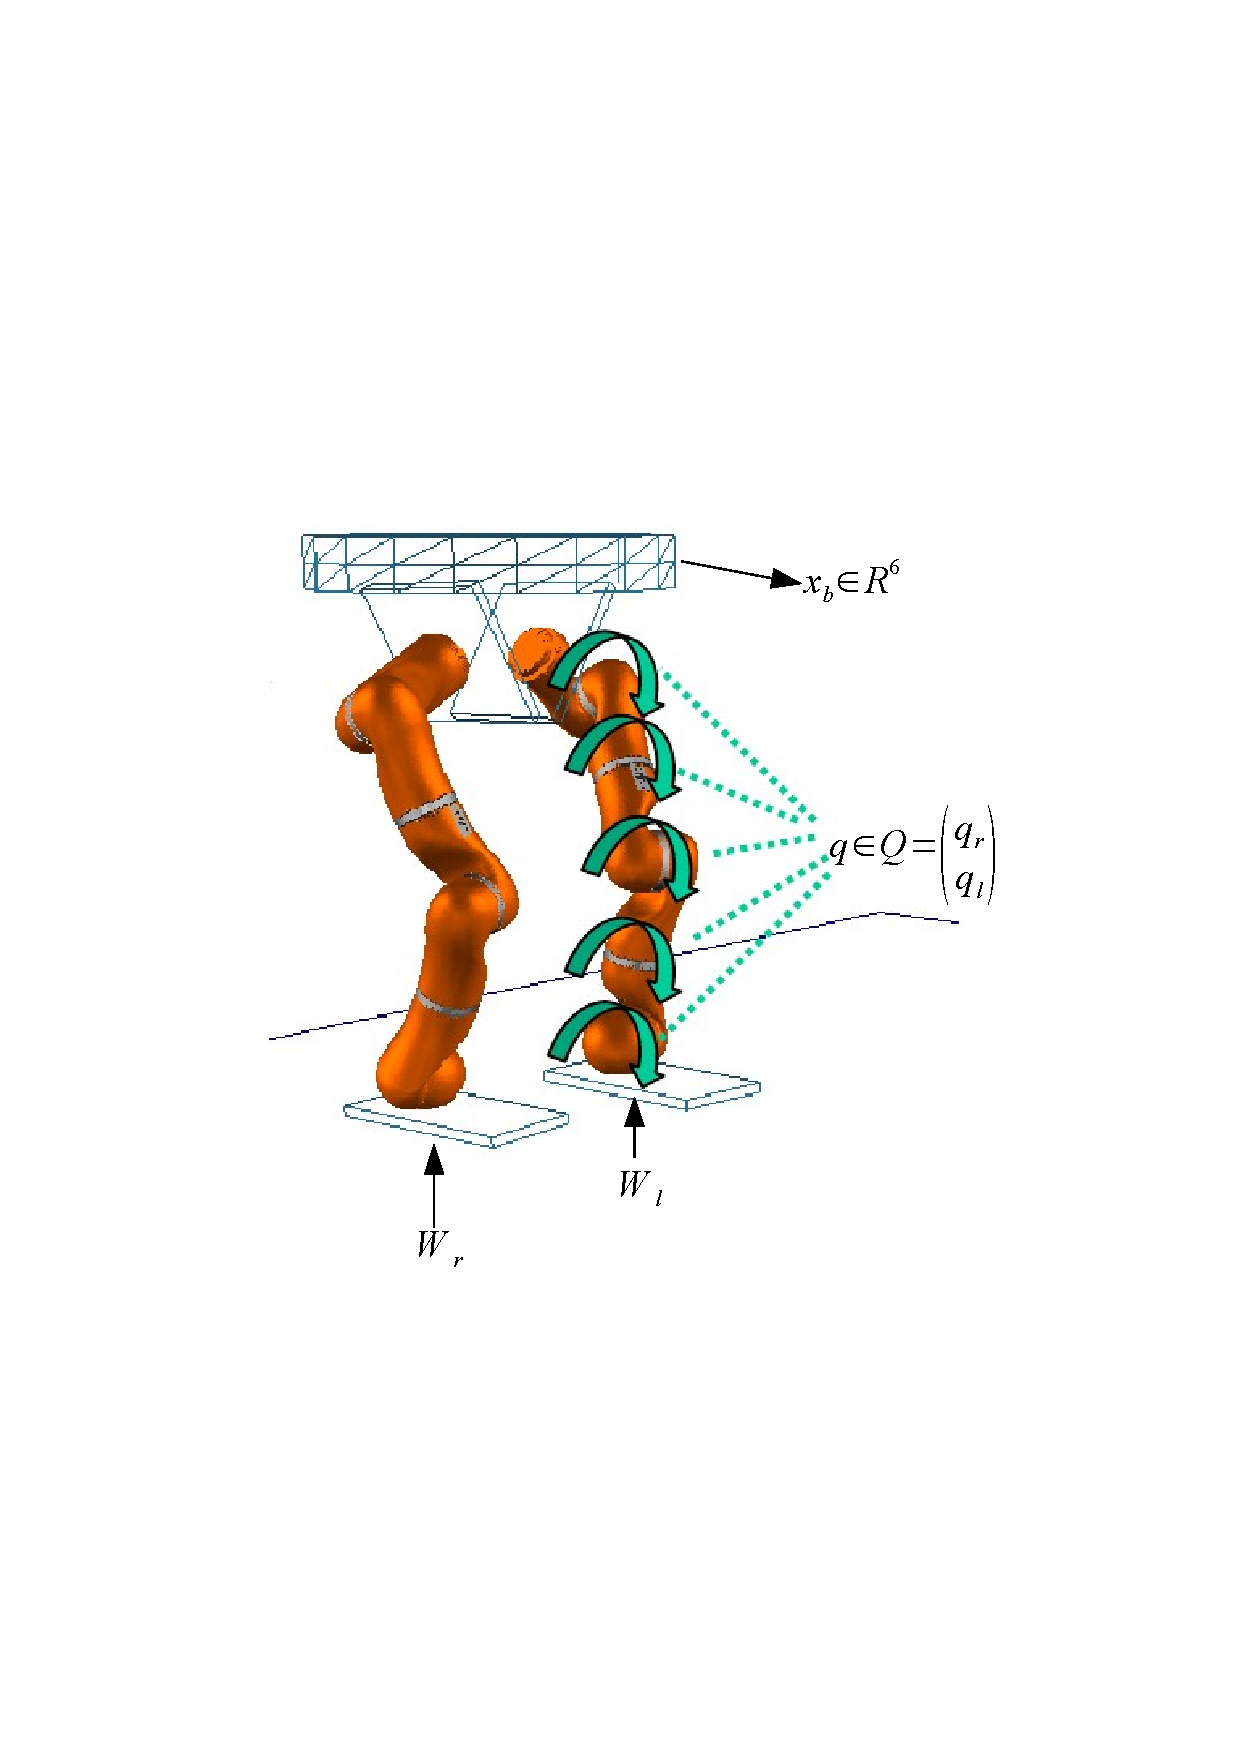
\includegraphics[trim= 10mm 80mm 10mm 80mm,scale=0.75]{Bilder/model_biped.pdf}
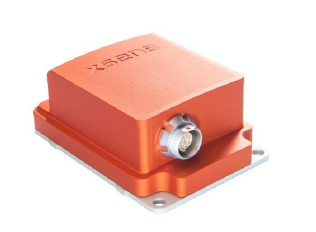
\includegraphics[scale=0.75]{Bilder/pic_imu.png}
\caption{IMU(\emph{MTi-100} mounted) on \emph{Toro}}
\label{fig:toro_imu}
\end{center}
\end{figure}
\begin{equation}
    \label{eq:imu_acc}
    a = R(a_{abs} - g),
\end{equation}
where $a_{abs} $ is the absolute acceleration of the body with respect to spatial frame (world frame) and \emph{g} denotes the acceleration due to gravity $[0,0,-9.81]^T$.

The measurement from the IMU are noisy. In addition to the noise there can be bias acting on the measurements. The stochastic model of the IMU is 
\begin{equation}
\label{eq:imu_noise}
\begin{split}
\tilde{a} &= a + b_a + w_a \\
\dot{b}_a &= w_{ba} \\
\tilde{\omega} &= \omega + b_\omega + w_\omega \\
\dot{b}_\omega &= w_{b\omega},
\end{split}
\end{equation}
where $\tilde{a}$ is the acceleration measured by the IMU. It is composed of true acceleration \emph{a}, bias $b_a$ and the sensor noise $w_a$. The measured angular velocity is $\tilde{\omega}$, true angular velocity $\omega$, bias $b_{\omega}$ and sensor noise $w_\omega$. The sensor noises $w_a$ and $w_\omega$ are modelled as zero mean Gaussian white noise. The biases $b_a$ and $b_\omega$ are dynamical quantities but they have very slow dynamics. The bias dynamics $\dot{b}_a$ and $\dot{b}_\omega$ are modelled as first order Markov process. The bias is driven by zero mean Gaussian white noises $w_{b\omega}$ and $w_{bf}$.

\subsection{State space representation}
The state space formulation of the dynamic model is based on Equation \ref{eq:fwdyn_ode}. Rearranging the Equation \ref{eq:imu_noise} in terms of true acceleration and true angular velocity and substituting Equation \ref{eq:imu_acc} in \ref{eq:imu_noise} leads to state space dynamic model. 
\begin{equation}
    \label{eq:dyn_imu}
    \begin{split}
    \dot{p} &= v \\
    \dot{v} &= a = R(\tilde{a} - b_a - w_a)+g \\
    \dot{\theta} &= T^{-1}\omega = T^{-1}(\tilde{\omega} - b_\omega - w_\omega) \\
    \dot{b}_a &= w_{ba}\\
    \dot{b}_\omega &= w_{b\omega}
    \end{split}
\end{equation}
\begin{itemize}
    \item $ r = \begin{bmatrix} p_x \\ p_y \\ p_z \end{bmatrix}$ is the position of IMU measurement frame with respect to spatial frame.
    \item $ v = \begin{bmatrix} v_x \\ v_y \\ v_z \end{bmatrix} = \begin{bmatrix} \dfdx{p_x}{t} \\ \dfdx{p_y}{t} \\ \dfdx{p_z}{t} \end{bmatrix}$ is the velocity of IMU measurement frame with respect to spatial frame.
    \item $ \theta = \begin{bmatrix} \theta_x \\ \theta_y \\ \theta_z \end{bmatrix}$ is the orientation of the IMU frame with respect to spatial frame. Orientation of IMU is parametrized as RPY Euler angles. $R=R(\theta)$ is the rotation matrix that rotates a vector in body coordinate frame to spatial coordinate frame. [Appendix \ref{sec:rot_mat}].
    \item $T=T(\theta)$ is the matrix that transforms angular rate $\dot{\theta}$ to angular velocity in the body frame $\omega$ [Appendix \ref{sec:avel_trfm}].
\end{itemize}
\begin{equation}
x = \begin{bmatrix} p \\ v \\ \theta \\ b_a \\ b_{b\omega} \end{bmatrix} \in \Re^{15}
\end{equation}

\subsection{Prediction step}
The prediction equations of EKF are given in Equation \ref{eq:ekf_predict}. For the sake of simplicity we assume the process noise acting on the model is uncorrelated. i.e The noise acting on each state is independent $$W_k = I_n$$. $n$ is the number of states. Substituting the value of $W_k$ in Equation \ref{eq:ekf_predict}
\begin{equation}
\label{eq:imu_predict}
\begin{split}
\hat{x}_{k+1}^- &= f(\hat{x}_{k},u_{k+1},0)\\
P_{k+1}^- &= A_kP_{k}A_k^T + Q_{k}\\
\end{split}
\end{equation}
The model is discretized for the implementation of EKF. Since the time step for integration is very small $\Delta t = 1ms$ forward Euler discretization method is used to discretize the continuous time model in \ref{eq:dyn_imu}.
\begin{equation}
    \label{eq:dyn_imu_disc}
    \begin{split}
    \hat{p}_{k+1}^- &= \hat{p}_k + \Delta t \hat{v}_k + \frac{\Delta t^2}{2} (\hat{R}_k (\tilde{a}_{k+1} - \hat{b}_{a,k})+g) \\
    \hat{v}_{k+1}^- &= \hat{v}_k + \Delta t (\hat{R}_k (\tilde{a}_{k+1} - \hat{b}_{a,k})+g) \\
    \hat{\theta}_{k+1}^- &= \hat{\theta}_k + \Delta t \hat{T}_k^{-1}(\tilde{\omega}_{k+1} - \hat{b}_{\omega,k+1}) \\
    \hat{b}_{a,k+1}^- &= \hat{b}_{a,k}\\\
    \hat{b}_{\omega,k+1}^- &= \hat{b}_{\omega,k}
    \end{split}
\end{equation}
The system matrix is obtained by computing the Jacobian of the discretized system of equations is
\begin{equation}
    A_k = \begin{bmatrix}
    I_3 &\Delta t &\frac{\Delta t^2}{2} \dfdx{\hat{R}_k}{\theta}(\tilde{a}_{k+1} - \hat{b}_{a,k} ) &-\frac{\Delta t^2}{2} \hat{R}_k &\textbf{0}_3 \\
    \textbf{0}_3 &I_3  &\Delta t \dfdx{\hat{R}_k}{\theta}(\tilde{a}_{k+1} - \hat{b}_{a,k} ) &-\Delta t\hat{R}_k &\textbf{0}_3\\
    \textbf{0}_3  &\textbf{0}_3 &I_3 + \Delta t \dfdx{\hat{T}^{-1}}{\theta}(\tilde{\omega}_{k+1} - \hat{b}_{\omega,k+1}) &\textbf{0}_3 &\Delta t \hat{T}_k^{-1}\\
    \textbf{0}_3  &\textbf{0}_3  &\textbf{0}_3  &I_3 &\textbf{0}_3 \\
    \textbf{0}_3  &\textbf{0}_3  &\textbf{0}_3  &\textbf{0}_3 &I_3
    \end{bmatrix}
\end{equation}

\subsection{Update step}
The update equation of the EKF is given in Equation \ref{eq:ekf_correct}. The measurement equation of the system is given by $$\hat{y}_{k+1} = h(\hat{x}_{k+1}^-,u_{k+1},0)$$.For the sake of simplicity let us assume the measurement of noise are independent. $$V_k = I_3$$. Substituting the assumption in \ref{eq:ekf_correct}
\begin{equation}
\label{eq:imu_correct}
\begin{split}
K_{k+1} &= P_{k+1}^-\hat{C}_{k+1}^{T}(\hat{C}_{k+1}P_{k+1}^-\hat{C}_{k+1}^{T} + R_{k+1})^{-1}\\
\hat{x}_{k+1} &= \hat{x}_{k+1}^- + K_{k+1}(y_{k+1}-\hat{y}_{k+1})\\
P_{k+1} &= (I- K_{k+1}\hat{C}_{k+1})P_{k+1}^-
\end{split}
\end{equation}
The contact points are the only measurements that are considered for the update step. Figure \ref{fig:biped_feet} shows the contact points. The Force torque sensor (FTS) measurement is used to compute the ZMP[Appendix \underline{Zero moment point}] of the foot and also to determine the foot that is in contact with the ground. The measurement equation is same as Equation \ref{eq:y_kin} of the multi body system model. $H_{RF} \text{ and } H_{LF} $ are formed as the composition of $H_{hip}^s H_{RF}^{hip}$ and $H_{hip}^s H_{RF}^{hip}$ respectively.
\begin{equation}
    \label{eq:imu_msr}
    \begin{split}
    y_{i,j} &= H(r,\theta) kin_j(q)p_i \hspace{2cm} \forall i=\{A,B,C,D\} \text{ and } j=\{RF,LF\} \\
    &= H_{hip}^s H_{foot}^{hip}p_i \\
    &= H p_{foot,i}^{hip}
    \end{split}
\end{equation}
\begin{itemize}
    \item $H(r,\theta)$ is the homogeneous transformation matrix of the frame attached to the IMU and the spatial frame [Appendix \ref{sec:htm}]
    \item $kin_j(q)$ computes the homogeneous transformation matrix of foot relative to hip. \emph{q} represents joint angles measured by encoders.
\end{itemize}
The measurement sensitivity matrix is computed by taking the Jacobian of the measurement equation.
\begin{equation}
        \hat{C}_{k+1} = \dfdx{\hat{y}_{k+1}}{x} = \dfdx{\hat{H}_{k+1}}{x} kin_j(q_{k+1}) p_i \hspace{1cm} \forall i=\{A,B,C,D\} \text{ and } j=\{RF,LF\} 
\end{equation}
\begin{itemize}
    \item $\dfdx{\hat{H}_{k+1}}{x}$ is the partial derivative of homogeneous transformation matrix with respect to system states. [Appendix \ref{sec:htm}]
\end{itemize}

% Experiments
\subsection{Experiment}

\begin{figure}
% We need layers to draw the block diagram
\pgfdeclarelayer{background}
\pgfdeclarelayer{foreground}
\pgfsetlayers{background,main,foreground}

% Define a few styles and constants
\tikzstyle{sensor}=[draw, fill=blue!20, text width=5em,text centered, minimum height=2.5em]
\tikzstyle{system} = [sensor, text width=6em, fill=green!30, 
    minimum height=12em, rounded corners]
\tikzstyle{input} = [coordinate]
\tikzstyle{sum} = [draw, fill=blue!20, circle, node distance=1cm]
%\tikzstyle{output} = [coordinate]
\def\blockdist{0.5}
\def\edgedist{0.75}
\begin{tikzpicture}
	% Define the nodes in the picture
	\node (sys_in)[yshift=1cm]{$x_0$};
	\node (u_in) [below of=sys_in,node distance=1cm]{$u$};
	\node (sys_u)[input,right of=u_in,node distance=1cm]{};
    \node (sim_sys) [system,right of=sys_in,node distance=3cm] {Double pendulum system};
    \node (sys_noise)[above of=sim_sys,node distance=3cm]{$n_w$};
    \node (msr_noise)[right of=sys_noise,node distance=2cm]{$n_v$};
    \node (msr_add)[sum,right of=sim_sys,node distance=2cm]{};
    \node (estimator) [system,right of=msr_add,node distance =3cm]{ Estimator};
    \node (est_in) [right of=sim_sys,node distance=3cm,yshift=1.5cm]{$\hat{x}_0$};
    \node (est_u) [input,right of =sim_sys, node distance=2cm,yshift=-3cm]{foo};
    \node (est_out)[right of=estimator,node distance=3cm]{$\hat{x}$};
    
    % Define the edges in the picture
    \draw [->] (sys_in) --node{}(sim_sys.west);
    \draw [-] (u_in) --node{}(sys_u);
    \draw [->] (sys_u) --node{}+(\edgedist,0);
    \draw [-] (sys_u) |-node{}(est_u);
    \draw [->] (est_u) |-node[pos=0.7,above]{$u$}(estimator.-130);
    \draw [->] (est_in) --node{}+(\edgedist,0);
    \draw [->] (sys_noise) --node{}(sim_sys.north);
    \draw [->] (msr_noise) --node{}(msr_add.north);
    \draw [->] (sim_sys.east) --node[above]{}(msr_add.west);
    \draw [->] (msr_add.east) --node[above]{$y$}(estimator.west);
    \draw [->] (estimator) --node{}(est_out);
\end{tikzpicture}
\caption{Experimental setup for the simple model}
\end{figure}


    \chapter{Conclusion}
\label{ch:conclusion}

%Filter Comparison:
 The state estimation problem is solved with the EKF and the UKF. The EKF involves more modeling than the UKF. For example modeling of the Jacobian matrices $A$ and $C$ for multibody model of \emph{Toro} in Chapter \ref{ch:multi_mdl}. The UKF is easier to tune for models with less number of states (IDP) than for the models with many states (\emph{toro}). The computation time of the UKF is higher than the EKF for all the models. 
 \begin{table}[H]
	\centering
	\setlength{\extrarowheight}{0.5cm}
%\setlength{\extrarowwidth}{0.1cm}
\begin{tabular}{|x{1cm}|x{2cm}|x{2.1cm}|}\hline
Model&RMSE&Computation time\\ \hline
IDP&\diag{0.25em}{2cm}{ 
\includegraphics[scale=0.025]{Bilder/thumbs-up.png} }{
\includegraphics[scale=0.025]{Bilder/thumbs-up.png}}&\diag{0.25em}{2cm}{
\includegraphics[scale=0.025]{Bilder/thumbs-up.png}}{
\includegraphics{Bilder/thumbs-down.png}} \\ \hline
Toro&\diag{0.25em}{2cm}{
\includegraphics[scale=0.025]{Bilder/thumbs-up.png}}{
\includegraphics{Bilder/thumbs-down.png}}&\diag{0.25em}{2cm}{
\includegraphics[scale=0.025]{Bilder/thumbs-up.png}}{
\includegraphics{Bilder/thumbs-down.png}}\\ \hline
IMU&\diag{0.25em}{2cm}{
\includegraphics[scale=0.025]{Bilder/thumbs-up.png}}{-}&\diag{0.25em}{2cm}{
\includegraphics[scale=0.025]{Bilder/thumbs-up.png}}{-}\\ \hline
\end{tabular}

	\caption{Comparison of qualitative performance of EKF and UKF on the models}
	\label{tab:comp_ekf_ukf}
\end{table}

The smiley \footnote{Smiley image source:\url{http://www.clker.com/}.} on the left side of each cell in Table \ref{tab:comp_ekf_ukf} refers to the performance of EKF, whereas the one on the right side of refers to UKF. Since the UKF was not developed for the IMU model the RMSE is left blank. 

%Models Comparison:
The state estimation problem is approached with multibody system model of \emph{Toro} and the model of IMU. The EKF has same performance with both models which can be inferred from the RMSE values of the estimates in Tables \ref{tab:toro_rmse} and \ref{tab:simp_rmse}. The computation time of EKF for the \emph{Toro} model is higher than the IMU model. This makes the \emph{Toro} model inapplicable for real time applications. Whereas the IMU model having low computation time is implemented on the real robot.

\begin{table}
	\centering
	%\setlength{\extrarowheight}{0.5cm}
	%\begin{tabular}{|x{1cm}|x{2cm}|x{2cm}|}\hline
	\begin{tabular}{|c|c|c|}\hline
	&Toro&IMU \\ \hline	
	RMSE &
\includegraphics[scale=0.025]{Bilder/thumbs-up.png}&
\includegraphics[scale=0.025]{Bilder/thumbs-up.png} \\ \hline
	Computation time &
\includegraphics{Bilder/thumbs-down.png} &
\includegraphics[scale=0.025]{Bilder/thumbs-up.png} \\ \hline
	\end{tabular}
	\caption{Comparison of qualitative performance of the models used in EKF }
\end{table}

The multibody model of \emph{Toro} is more descriptive and complicated than the IMU model. It is possible to estimate additional motion parameters like joint velocities $\dot q$ with this model, but it is computationally costly. This model is prone to modeling errors. The IMU model is simpler than multibody model and computationally cheap. The formulation of the model is easier than \emph{Toro} model. This model have the same performance as the \emph{Toro} model.

\subsection{Future works}
The filters designed in this thesis are aimed to be used in the controllers for balancing applications in \emph{Toro}. But this can be extended for walking applications in the future. The camera present at the head of \emph{Toro} provides measurements at lower frequency (100Hz) than the other sensors (1kHz). The could be incorporated as additional measurement \citep{vis12}.
    \chapter{Appendix}
\section{Symbols}
\label{sec:symbols}
\begin{tabular}{p{2cm} l}
$I_{x}$ & Identity matrix of dimension \emph{x} \\
$\textbf{0}_{r \times c}$ & Zero matrix of dimensions given by \emph{r,c}. \\
						  & \emph{r} - row dimension , \emph{c} - colomn dimension \\
$e_i$ 			& Unit vectors pointing in direction of the coordinate axis  \\
				& $e_1 = \begin{bmatrix} 1 \\ 0 \\ 0 \end{bmatrix} $ - unit vector along x axis \\						& $e_2 = \begin{bmatrix} 0 \\ 1 \\ 0 \end{bmatrix} $ - unit vector along y axis \\						& $e_3 = \begin{bmatrix} 0 \\ 0 \\ 1 \end{bmatrix} $ - unit vector along z axis \\	
$l_{m,n}$    	& Zero vector of length \emph{m}, with 1 in \emph{nth} position of the vector \\
			    & For Example, $l_{4,2} = \begin{bmatrix} 0 \\ 1 \\ 0 \\ 0 \end{bmatrix}, l_{2,1} = 						\begin{bmatrix} 1 \\ 0 \end{bmatrix} $ \\		
\end{tabular}

\section{Abbreviation}
\begin{tabular}{c l}
EKF & Extended Kalman filter \\
IMU & Inertial measurement Unit \\
FTS & Force torque sensor \\
ODE & Ordinary differential equation\\
ZMP & Zero moment point\\
RPY & Roll-Pitch-Yaw
\end{tabular}

\section{Rotation matrix}
\label{sec:rot_mat}
The orientation of a rigid body in space can be represented in form of rotational matrix $R \in SO(3)$. 
\begin{figure}
    \centering
    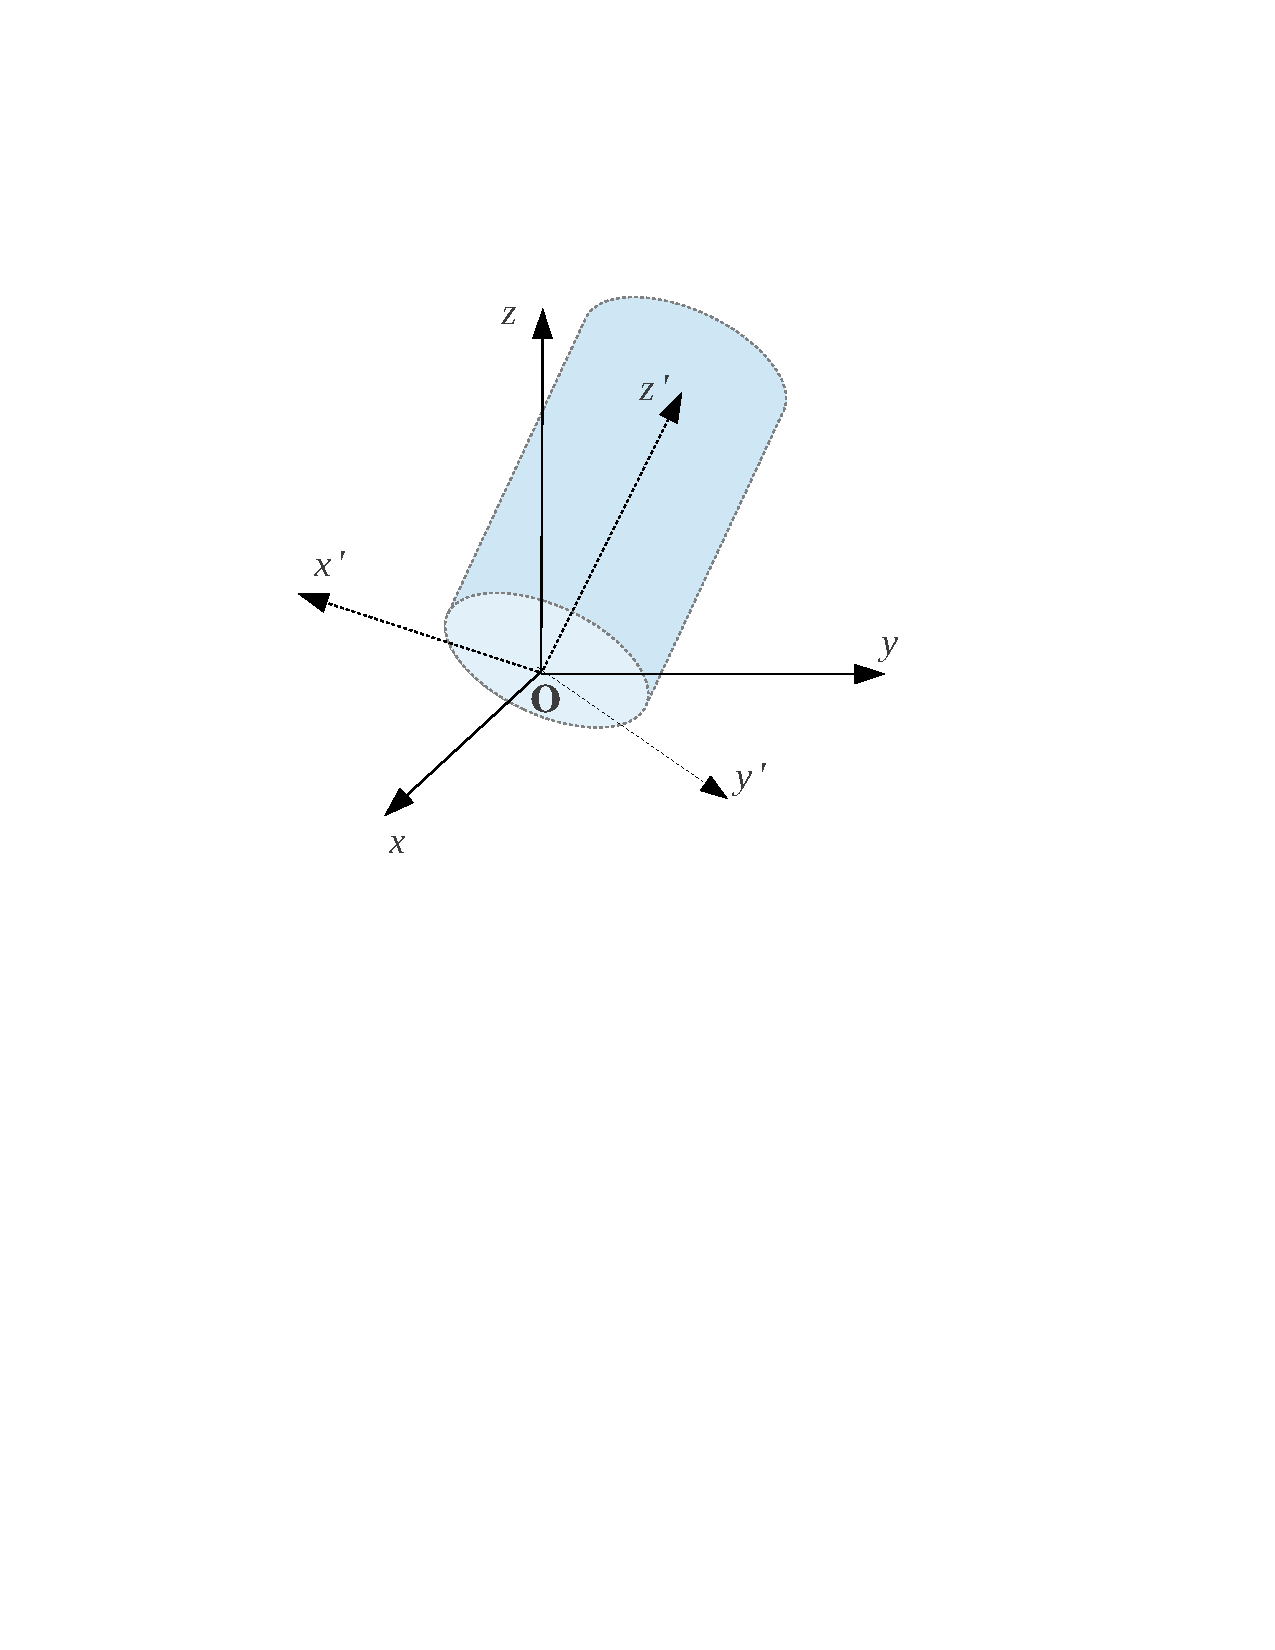
\includegraphics[trim = 5cm 13cm 5cm 5cm, scale = 0.65]{Bilder/rot_ab.pdf}
    \caption{Rotation of a rigid body about a point}
    \label{fig:rot_ab}
\end{figure}
Figure \ref{fig:rot_ab} shows the cylindrical object rotated about point \textbf{O}. \emph{x',y',z'} are the frames attached to the cylindrical object. The frame attached to the body of the object is denoted as frame \emph{B} \emph{x,y,z} represents the inertial frame or spatial frame and it is denoted as frame \emph{A}. The rotation of frame \emph{B} with respect to frame \emph{A} is given as $$ R_b^a.$$. In this thesis unless explicitly mentioned the rotation matrix represents the rotation of a body with respect to inertial frame or spatial frame. For the sake of simplicity in symbols the rotation of the body with respect to spatial frame is represented as $R$ instead of $R_b^a$.
A 3 dimensional rotation matrix defines the rotation along \emph{X,Y,Z} directions. The rotation matrix is composition of these individual rotations. The matrix representing the rotation around each coordinate axis is,
\begin{equation}
	\begin{split}
	R_x(\theta_x) = 
	\begin{bmatrix}
	1 &0 &0 \\ 0 &cos(\theta_x) &-sin(\theta_x)\\ 0 &sin(\theta_x) &cos(\theta_x)
	\end{bmatrix}\\
	R_y(\theta_y) = 
	\begin{bmatrix}
	cos(\theta_y) &0 &sin(\theta_y) \\ 0 &1 &0\\ -sin(\theta_y) &0 &cos(\theta_y)
	\end{bmatrix}\\
	R_z(\theta_z) = 
	\begin{bmatrix}
	cos(\theta_z) &-sin(\theta_z) &0 \\ sin(\theta_z) &cos(\theta_z) &0)\\ 0 &0 &1
	\end{bmatrix}
	\end{split}
\end{equation}
\begin{enumerate}
\item Rotation matrix for the whole body model in Chapter \ref{chap:multi_mdl} is 
\begin{equation}
	\label{eq:rot_full}
	\begin{split}
	R &= R_x(\theta_x) R_y(\theta_y) R_z(\theta_z) \\
	&= 
	\begin{bmatrix}
		c_yc_z &-c_ys_z &s_y \\
		c_xs_z+c_zs_xs_y &c_xc_z-s_xs_ys_z &-c_ys_x \\
  		s_xs_z-c_xc_zs_y &c_zs_x-c_xs_ys_z & c_xc_y \\
	\end{bmatrix}
	\end{split}
\end{equation}
The partial derivative of the above rotational matrix with respect to the angles is
\begin{equation}
	\begin{split}
	\dfdx{R}{\theta_x} &=
	\begin{bmatrix} 
		0 &0 &0 \\
        c_xs_yc_z-s_xs_z &-c_xs_ys_z-s_xc_z &c_xc_y]\\
        s_xs_yc_z+c_xs_z &-s_xs_ys_z+c_xc_z &-s_xc_y
	\end{bmatrix}\\
	\dfdx{R}{\theta_y}&=
	\begin{bmatrix}
    -s_yc_z &s_ys_z &c_y \\
     s_xc_yc_z &-s_xc_ys_z & s_xs_y \\
    -c_xc_yc_z & c_xc_ys_z &-c_xs_y
	\end{bmatrix}\\
	\dfdx{R}{\theta_z}&=
	\begin{bmatrix}
    -c_ys_z &-c_yc_z &0 \\
    -s_xs_ys_z+c_xc_z &-s_xs_yc_z-c_xs_z &0 \\
     c_xs_ys_z+s_xc_z &c_xs_yc_z-s_xs_z &0
	\end{bmatrix}
	\end{split}
\end{equation}
\item Rotation matrix for the simplified model in Chapter \ref{chap:simp_mdl} is parameterized as RPY angles
\begin{equation}
	\label{eq:rot_simp}
	\begin{split}
		R &= R_z(\theta_z) R_y(\theta_y) R_x(\theta_x)\\ &=
		\begin{bmatrix}
		c_zc_y &-s_zc_x+c_zs_ys_x &s_zs_x+c_zs_yc_x\\
		s_zc_y &c_zc_x+s_zs_ys_x &-c_zs_x+s_zs_yc_x\\
		-s_y &c_ys_x &c_yc_x
		\end{bmatrix}
	\end{split}
\end{equation}
The partial derivative of the above rotational matrix with respect to the angles is
\begin{equation}
	\begin{split}	
		\dfdx{R}{\theta_x} &=
		\begin{bmatrix}
		0 &s_zs_x+c_zs_yc_x &s_zc_x-c_zs_ys_x \\
		0 &-c_zs_x+s_zs_yc_x &-c_zc_x-s_zs_ys_x \\
		0 &c_yc_x &-c_ys_x
		\end{bmatrix}\\
		\dfdx{R}{\theta_y} &=
		\begin{bmatrix}
		-c_zs_y &c_zc_ys_x &c_zc_yc_x \\
		-s_zs_y &s_zc_ys_x &s_zc_yc_x \\
		-c_y &-s_ys_x &-s_yc_x
		\end{bmatrix}\\
		\dfdx{R}{\theta_z} &=
		\begin{bmatrix}
		-s_zc_y &-c_zc_x-s_zs_ys_x &c_zs_x-s_zs_yc_x \\
		c_zc_y &-s_zc_x+c_zs_ys_x &s_zs_x+c_zs_yc_x\\
		0 &0 &0
		\end{bmatrix}
	\end{split}
\end{equation}
\begin{itemize}
\item $ \theta_x, \theta_y, \theta_z $ represents the rotation of the body coordinate frame relative to spatial frame coordinate frame.
\item $ c_x,c_y,c_z $ are the short hand notations of $cos(\theta_x), cos(\theta_y), c_z$ respectively.
\item $ s_x,s_y,s_z $ are the short hand notations of $sin(\theta_x), sin(\theta_y), sin(\theta_z)$ respectively.
\end{itemize}
\end{enumerate}
\section{ Homogeneous transformation matrix}
\label{sec:htm}
Homogeneous transformation matrix is a one form of representation of rigid body transformation. It represents the transformation of a rigid body from the body coordinate frame to another cooridnate frame. 
\begin{figure}
    \centering
    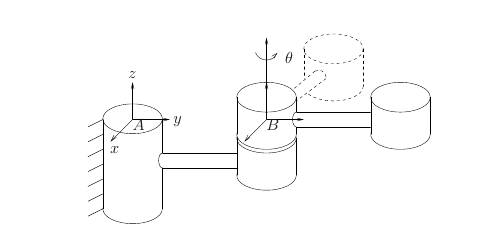
\includegraphics{Bilder/htm_example.png}
    \caption[Rigid body motion generated by rotation about a fixed axis]{Rigid body motion generated by rotation about a fixed axis \footnotemark[1]}
    \label{fig:htm}
\end{figure}
\footnotetext[1]{Source: A mathematical introduction to rigid body manipulation \citep[Chapter 2]{mur94}}
Homogeneous transformation matrix of body frame \emph{B} with respect to fixed frame \emph{A} is given as
\begin{equation}
    H_b^a = \begin{bmatrix} R_b^a(\theta) & p_{ab} \\ \textbf{0}_{3,1} &1 \end{bmatrix} \in SE(3),
\end{equation}
where $H_b^a$ represents the rigid body transfrormation of frame \emph{b} with respect to frame \emph{a}.
\begin{itemize}
    \item $R_b^a(\theta)$ is the rotation matrix representing rotation of body frame \emph{B} with respect to frame \emph{A}. 
    \item $p_{ab} = \begin{bmatrix} p_x \\ p_y \\ p_z \end{bmatrix} = \begin{bmatrix} p_1 \\ p_2 \\ p_3 \end{bmatrix} $ is the position of the body frame relative to spatial frame. 
\end{itemize}
For the sake of simplicity the homogeneous transofrmation matrix of a body with respect to spatial frame is represented by $H$ instead of $H_b^a$, the position as $p$ and rotation matrix as $R$.
The partial derivative of homogeneous transformation matrix with respect to poition and orientation.
\begin{equation}
    \begin{split}
    \dfdx{H}{p_i} &= \begin{bmatrix} \textbf{0}_{3,3} &e_i \\ \textbf{0}_{1,3} &1 \end{bmatrix} \hspace{2cm} i={1,2,3} \\
    \dfdx{H}{\theta_i} &= \begin{bmatrix} \dfdx{R}{\theta_i} &\textbf{0}_{3,1} \\ \textbf{0}_{1,3} &1 \end{bmatrix}
    \end{split}
\end{equation}

\section{Transformation of angular velocity to Euler rates}
\label{sec:avel_trfm}
The relation between the angular velocity and time derivative of rotational matrix is $$ \omega^b = (R^T \dot{R}) ^ \vee $$
\begin{itemize}
\item $\omega^b$ is the angular velocity of the body in represented in body coordinate frame. 
\item $R^T \dot{R}$ is a skew symmetric matrix \citep[Chapter 2]{mur94}.
$$ R^T \dot{R} = \begin{bmatrix}
0 &-\omega_z^b &\omega_y^b\\ \omega_z^b &0 &-\omega_x^b \\ -\omega_y^b &\omega_x^b &0 \end{bmatrix}$$
\item $\vee$ operator extracts the 3 dimensional vector that forms the skew symmetric matrix
$$ (R^T \dot{R}) ^ \vee = \begin{bmatrix}\omega_x^b\\ \omega_y^b\\ \omega_z^b \end{bmatrix} = w^b$$
\end{itemize}
The rotation matrix R is parametrized by Euler angles. $w^b$ depends on the parametrization of the rotation matrix.
\begin{enumerate}
\item For the whole body model discussed in Chapter \ref{chap:multi_mdl} the rotation matrix is given in Equation \ref{eq:rot_full}. The angular velocity is
\begin{equation}
	\begin{split}
	\omega_x^b &= cos(\theta_z)cos(\theta_y)\dot{\theta}_x + sin(\theta_z)\dot{\theta}_y \\
	\omega_y^b &= - sin(\theta_z)cos(\theta_y)\dot{\theta}_x + cos(\theta_z)\dot{\theta}_y \\
	\omega_z^b &= sin(\theta_y)\dot{\theta}_x + \dot{\theta}_z \\
	\begin{bmatrix}
	\omega_x^b\\ \omega_y^b\\ \omega_z^b
	\end{bmatrix}
	 &= 
	\begin{bmatrix}
		cos(\theta_z)cos(\theta_y) &sin(\theta_z) &0 \\
	 	-sin(\theta_z)cos(\theta_y) &c_z&0 \\
		sin(\theta_y) &0 &1
	\end{bmatrix}
	\begin{bmatrix}
			\dot{\theta_x} \\ \dot{\theta_y}\\ \dot{\theta_z}
	\end{bmatrix}\\
	& \omega^b = T(\theta) \dot{\theta}
	\end{split}
\end{equation}
$T(\theta)$ is the transformation matrix, that transforms the time derivative of euler angles parametrized in Equation \ref{eq:rot_full}.

The partial derivatives of $\omega^b$ with respect to the states are
$$\dfdx{\omega_b}{\theta_x} = \textbf{0}_{3\times 3},\dfdx{\omega_b}{\theta_y} = \begin{bmatrix}	-c_zs_y &0 &0\\ s_zs_y &0 &0\\ c_y &0 &0 \end{bmatrix}, \dfdx{\omega_b}{\theta_z} = \begin{bmatrix}	-s_zc_y &c_z &0\\ -c_zc_y &-s_z &0\\ 0 &0 &0 \end{bmatrix} $$

\item For the simple model discussed in Chapter \ref{chap:simp_mdl} the rotation matirx is given in Equation \ref{eq:rot_simp}. The angular velocity is
\begin{equation}
	\begin{split}
	\omega_x^b &= \dot{\theta}_x - sin(\theta_y)\dot{\theta}_z \\
	\omega_y^b &= cos(\theta_x)\dot{\theta}_y + cos(\theta_y)sin(\theta_x)\dot{\theta}_z \\
	\omega_z^b &= -sin(\theta_x)\dot{\theta}_y + cos(\theta_y)cos(\theta_x)\dot{\theta}_z \\
	\begin{bmatrix}
	\omega_x^b\\ \omega_y^b\\ \omega_z^b
	\end{bmatrix}
	 &= 
	\begin{bmatrix}
	 &1 &0 &-s_y\\
	 &0  &c_x &c_ys_x\\
	 &0  &-s_x &c_yc_x
	\end{bmatrix} \\
	&\omega^b = T(\theta) \dot{\theta}
	\end{split}
\end{equation}
$T(\theta)$ is the transformation matrix, that transforms the time derivative of euler angles parametrized in Equation \ref{eq:rot_simp}.

The partial derivatives of $\omega^b$ with respect to the states are
$$\dfdx{\omega_b}{\theta_y} = \begin{bmatrix}0 &0 &0\\ 0 &-s_x &c_yc_x\\ 0 &-c_x &-c_ys_x \end{bmatrix}, \dfdx{\omega_b}{\theta_z} = \begin{bmatrix}0 &0 &-c_y\\ 0 &0 &-s_ys_x\\ 0 &0 &-s_yc_x \end{bmatrix},\dfdx{\omega_b}{\theta_z} = \textbf{0}_{3\times 3} $$
\end{enumerate}



    %%%%%%%%%%
    % Anhang %
    %%%%%%%%%%

    \appendix
	%\printindex
    %Abbildungsverzeichnis
    \listoffigures
    \addcontentsline{toc}{chapter}{List of figures}
    %\addcontentsline{lof}{figure}{List of figures}
    \cleardoublepage
    %list of tables
    %\listoftables
    %\addcontentsline{lot}{tables}{List of tables}
    % Literaturverzeichnis
    \addcontentsline{toc}{chapter}{\bibname}
    %\bibliographystyle{gerplain}
    %\bibliographystyle{unsrt}
    \bibliographystyle{alphadin}
    %\bibliography{literatur}
    \bibliography{thesis}
    % To complie succesfully wit bibtex use the following sequence of operation
    % F1 -> F11 -> F1 -> F1
    		
    % Erklaerung
    \newpage
    \thispagestyle{myheadings}
    \markboth{}{ERKL\"{A}RUNG}
    \addcontentsline{toc}{chapter}{Erkl\"{a}rung}
    % erklaerung.tex
% Stand 31.08.2011

\cleardoublepage
\begin{center}
\textbf{Eidesstattliche Versicherung}
\end{center}
\normalsize
% Eventuell anzupassen
%\vspace{2cm}
\begin{table}[H]
	\begin{tabular}{p{10cm} p{5cm}}
	\underline{Rajendran, Rajesh} & 	\underline{146073\hspace{1cm}} \\
	Name, Vorname  &Matrikel-Nr.
	\end{tabular}
\end{table}
Ich versichere hiermit an Eides statt, dass ich die vorliegende \underline{Masterarbeit} mit dem Titel \\
\begin{center}
\textbf{\underline{"Estimation of underactuated degrees of freedom in humanoid robots"}}
\end{center}
%\hrulefill \\ \hrule \hrule
%\hrulefill \\ \hrule  \hrule
\vspace{0.5cm}
selbstst�ndig und ohne unzul�ssige fremde Hilfe erbracht habe. Ich habe keine anderen als die angegebenen Quellen und Hilfsmittel benutzt sowie w�rtliche und sinngem��e Zitate kenntlich gemacht. Die Arbeit hat in gleicher oder �hnlicher Form noch keiner Pr�fungsbeh�rde vorgelegen.\\
%\vspace{2cm}
\normalsize
\begin{table}[H]
	\begin{tabular}{p{10cm} p{5cm}}
	\underline{Dortmund,den \today} & 	\underline{\hspace{3cm}} \\
	Ort, Datum  &Unterschrift.
	\end{tabular}
\end{table}

\textbf{Belehrung:} 

Wer vors�tzlich gegen eine die T�uschung �ber Pr�fungsleistungen betreffende Regelung einer Hochschulpr�fungsordnung verst��t, handelt ordnungswidrig. Die Ordnungswidrigkeit kann mit einer Geldbu�e von bis zu 50.000,00 Euro geahndet werden. Zust�ndige Verwaltungsbeh�rde f�r die Verfolgung und Ahndung von Ordnungswidrigkeiten ist der Kanzler der Technischen Universit�t Dortmund. Im Falle eines mehrfachen oder sonstigen schwerwiegenden T�uschungsversuches kann der Pr�fling zudem exmatrikuliert werden. (� 63 Abs. 5 Hochschulgesetz - HG - )\\

Die Abgabe einer falschen Versicherung an Eides statt wird mit Freiheitsstrafe bis zu 3 Jahren oder mit Geldstrafe bestraft.\\

Die Technische Universit�t Dortmund wird gfls. elektronische Vergleichswerkzeuge (wie z.B. die Software "turnitin") zur �berpr�fung von Ordnungswidrigkeiten in Pr�fungsverfahren nutzen.\\

Die oben stehende Belehrung habe ich zur Kenntnis genommen:\\
\begin{table}[H]
	\begin{tabular}{p{10cm} p{5cm}}
	\underline{Dortmund,den \today} & 	\underline{\hspace{3cm}} \\
	Ort, Datum  &Unterschrift.
	\end{tabular}
\end{table}
\begin{comment}
%Hiermit best�tige ich, die vorliegende Diplomarbeit selbst�ndig und nur unter Zuhilfenahme
%der angegebenen Literatur verfasst zu haben.
\setlength{\parskip}{50pt}
\par
% In manchen Studieng�ngen optional. Gegebenenfalls l�schen.
Ich bin damit einverstanden, dass Exemplare dieser Arbeit in den Bibliotheken der
Universit�t Dortmund ausgestellt werden. 
\setlength{\parskip}{50pt}
\par
Dortmund, den \today 
\setlength{\parskip}{50pt}
\par
Name
\end{comment}
\clearpage
% EOF

%%%%%%%
% END %
%%%%%%%
\end{document}



